% IEEEtran uses legacy font families; select their encoding before class loading.
\RequirePackage[T1]{fontenc}
\documentclass[10pt,journal,compsoc]{IEEEtran}

\ifCLASSOPTIONcompsoc
  \usepackage[nocompress]{cite}
\else
  \usepackage{cite}
\fi
\usepackage{amsmath,amssymb,amsfonts}
\usepackage{tabularx}
\usepackage{booktabs}
\usepackage{graphicx}
\usepackage{textcomp}
\usepackage{courier}
\usepackage{xcolor}
\usepackage{float}
\usepackage{url}
\usepackage{diagbox}
\usepackage{makecell}
\usepackage{subfigure}
\usepackage{colortbl}
\definecolor{zigbeebg}{RGB}{251,227,227} % light Zigbee red
\definecolor{zwavebg}{RGB}{223,235,250}  % light Z-Wave blue
\definecolor{rqcolor}{RGB}{0,102,204} % vivid blue for research-question labels

\hyphenation{op-tical net-works semi-conduc-tor}

\newcommand{\system}{\textsc{AutoVD}}
\DeclareRobustCommand{\rq}[1]{\textcolor{rqcolor}{\textbf{RQ#1}}}
\newcommand{\parab}[1]{\vspace{0.04in}\noindent\textbf{#1}}
\newcommand{\todo}[1]{\textcolor{red}{[TODO: #1]}}

\begin{document}

\title{\system{}: State-Conditioned Black-Box Fuzzing of IoT Devices with LLM Agents}
\author{Anonymous Authors}
\markboth{Under Submission}{Anonymous Authors: \system}

\IEEEtitleabstractindextext{%
\begin{abstract}
Vulnerabilities in Internet of Things (IoT) devices may be triggered only by specific combinations of protocol messages and device configurations. Existing state-aware fuzzers provide limited support for verifying execution conditions and preserving them across test reuse. Their feedback also overlooks intermediate progress and earlier actions contributing to delayed failures. To address these issues, we present \system{}, an agent-guided black-box fuzzing framework for state-dependent vulnerability discovery. Large language model (LLM) agents combine message relationships and device attributes to plan mutation sequences, verify preconditions, and adapt tests to execution feedback. Conditional memory retains executable setup and applicability conditions for reuse across device-state changes. Progress-aware feedback and replay-supported sequence credit guide two-level scheduling and associate delayed failures with earlier decisions. Evaluation on 14 Zigbee and Z-Wave devices identifies 37 vulnerabilities, including 31 zero-days, with 7 CVEs assigned. Compared with ZVDetector, \system{} discovers more vulnerabilities in less time. It also achieves broader coverage of validated message formats, message relationships, and device attributes than the evaluated baselines.

\end{abstract}
\begin{IEEEkeywords}
vulnerability detection, IoT stateful fuzzing, black-box fuzzing, large language models, multi-agent systems
\end{IEEEkeywords}}

\maketitle
\IEEEdisplaynontitleabstractindextext
\IEEEpeerreviewmaketitle

\IEEEraisesectionheading{\section{Introduction}\label{sec:introduction}}

\IEEEPARstart{I}{nternet} of Things (IoT) devices process protocol messages whose effects depend on earlier exchanges and the device's current configuration. A message that is harmless in one state may expose a defect after a particular setup or sequence. Commercial devices rarely expose enough firmware information for instrumentation, so a tester must infer these conditions through the protocol interface. Mutating a valid packet is therefore only part of the problem: the tester must also reach the state in which the mutation matters.

Firmware analysis offers complementary ways to investigate such defects. Static methods recover data flows and validation constraints from binaries~\cite{karonte,satc,mango,nuwa}. Rehosting-based fuzzers obtain execution coverage by modeling the firmware environment~\cite{firmafl,fuzzware,hoedur}. These approaches depend on firmware access or an executable model of the target. Black-box testing instead interacts with a running device, making it suitable when firmware recovery and instrumentation are unavailable. Its weaker observations, however, make progress and failure attribution harder to establish.

Large language models (LLMs) help fuzzers interpret protocol specifications and execution responses. LLMIF uses response reasoning to enrich useful sequences~\cite{llmif}, while mGPTFuzz derives state machines and checks attribute observations for non-crash bugs~\cite{mgptfuzz}. MALF introduces coordinated agent planning and historical retrieval~\cite{malf}. ZVDetector discovers message relationships and command-accessible device attributes to explore combined protocol and device states~\cite{zvdetector}. These capabilities provide a starting point for stateful testing. The unresolved design question is how a continuing campaign preserves a test's applicability and learns from outcomes that become visible later.

Consider a state-dependent bulb failure involving correlated Groups/Scenes operations~\cite{zvdetector}. Clearing the group table and executing these operations precede a crash exposed by a later query. The query identifies where the failure becomes observable, but does not capture the mutation or its prerequisites. A payload-only seed loses the sequence that exercises it, and even a complete sequence can become inapplicable after the initial state changes. Meanwhile, ordinary exchanges along the path may extend exploration without producing an immediate anomaly. The testing process thus needs both condition-preserving experience and feedback that distinguishes reaching useful behavior from observing a fault.

\parab{Our approach.}
We organize \system{} around a \emph{state-conditioned test} that binds an ordered sequence and its mutation objective to a compatible target and checked initial conditions. This representation connects semantic planning to actual device behavior. The Mutator jointly selects the protocol prefix and device setup needed to exercise a mutation. Before execution, a Result Checker verifies supported operations and declared mutation intent. Runtime observations then establish whether the required state was reached. This boundary preserves deliberately malformed tests while preventing incidental construction errors or stale state assumptions from being mistaken for evidence about the chosen hypothesis.

The same test representation governs reuse and feedback. Long-term memory retains the setup, applicability conditions, and reproduction evidence needed to revisit useful sequences. The Evaluator provides bounded progress for validated state expansion before a security event occurs. When a delayed event is confirmed, replay supports redistribution of one event budget to relevant earlier choices. Updating the utilities of the original experiments leaves their trial counts unchanged. A two-level upper confidence bound (UCB) scheduler uses these utilities to select state--message opportunities and then compare mutations within the chosen context. The scheduler allocates exploration effort, while the Evaluator determines feedback from execution evidence.

\parab{Contributions.}
\begin{itemize}
  \item \textbf{Tool-driven agent testing.} We present an agent-guided black-box fuzzing framework for the combined space of protocol and device states. Tool-supported planning connects message sequences to relevant device preconditions, and execution feedback guides subsequent choices. The testing loop operates autonomously within configured access and recovery limits without requiring firmware source code.
  \item \textbf{Unified state awareness.} We combine semantic analysis with active verification to identify message dependencies and correlations for protocol-state graph exploration. Three-stage, multi-source analysis identifies basic, vendor-specific, and command-observable hidden attributes together with their types and access methods. These complementary views support joint sequence generation and device-state preparation, including functional commands that change otherwise read-only attributes.
  \item \textbf{Condition-preserving hierarchical memory.} We separate current runtime observations from role-specific short-term memory and structured long-term experience. High-value payloads and replayable sequences retain compatible device profiles, initial predicates, and reproduction evidence. Compact dynamic context and on-demand retrieval support cross-session reuse without treating historical observations as current state or injecting the full campaign history.
  \item \textbf{Deterministic long-horizon feedback and two-level scheduling.} We separate event severity, bounded observable progress, and replay-supported sequence contribution. Confirmed events supply one conserved credit budget, and an idempotent ledger revises earlier utilities without adding trials. Two-level UCB schedules state--message opportunities and context-specific mutations, while separate frontier and replay budgets support continued exploration and anomaly investigation.
  \item \textbf{Experimental evaluation.} We evaluate \system{} on 14 Zigbee and Z-Wave devices from eight vendors. Our experiments uncover 37 vulnerabilities, including 31 zero-days, with 7 CVE IDs assigned. Furthermore, agent-generated test cases can expose device vulnerabilities faster and uncover more state-dependent corner cases.\footnote{We release all source code at \url{https://github.com/colinLH/IoT-VDA/tree/main}.}
\end{itemize}

\section{Motivations, Challenges and Threat Model}\label{sec:motivation}
Stateful black-box testing must reach the conditions under which a mutation matters, preserve them when reusing experience, and interpret outcomes that become visible later. A smart-bulb vulnerability, CVE-2024-51384, illustrates these requirements. We identify three motivations and their corresponding challenges, then outline the solutions and define the threat model.

\subsection{Motivating Examples}\label{sec:examples}
\parab{A mutation whose effect depends on an earlier state.}
Figure~\ref{fig:state-example}(a) illustrates CVE-2024-51384, a state-dependent denial-of-service vulnerability in the Tuya TS0505B smart bulb that involves related Groups and Scenes operations~\cite{zvdetector}. The test first sends \emph{RemoveAllGroups} to establish the hidden attribute \texttt{group\_count}=0. It then sends \emph{AddGroup} with an excessively long group name and preserves the group identifier shared by the subsequent \emph{AddScene} and \emph{GetSceneMembership}. The final scene-membership query exposes a crash that requires a reboot. The query marks the observation point, but the test also includes the earlier state preparation and correlated messages. Testing only the final query would omit the context in which the failure is observed.

\parab{Revisiting the sequence after a restart.}
Figure~\ref{fig:state-example}(b) illustrates a campaign that records the CVE trace and later resumes after a restart. Retaining only the mutated name loses the setup and shared identifiers. Retaining all packet bytes still does not establish whether the target is compatible or the group table is empty in the new session. Useful reuse therefore requires both the recorded experiment and fresh checks of its preconditions. The restart scene is a derived testing situation, not a measured restart experiment.

\parab{Learning before the final alarm.}
As Figure~\ref{fig:state-example}(c) shows, the exchanges preceding the query return normal responses even as they establish a useful condition or extend the explored path. Zero feedback for all such exchanges gives the scheduler no distinction between progress and a familiar loop. A constant positive reward instead makes repeated normal traffic indefinitely valuable. When the crash eventually becomes visible, rewarding only the query overlooks earlier choices, whereas crediting every message equally also rewards unrelated traffic. This feedback situation illustrates the design problem rather than a measured AutoVD trace.

\begin{figure*}[t]
  \centering
  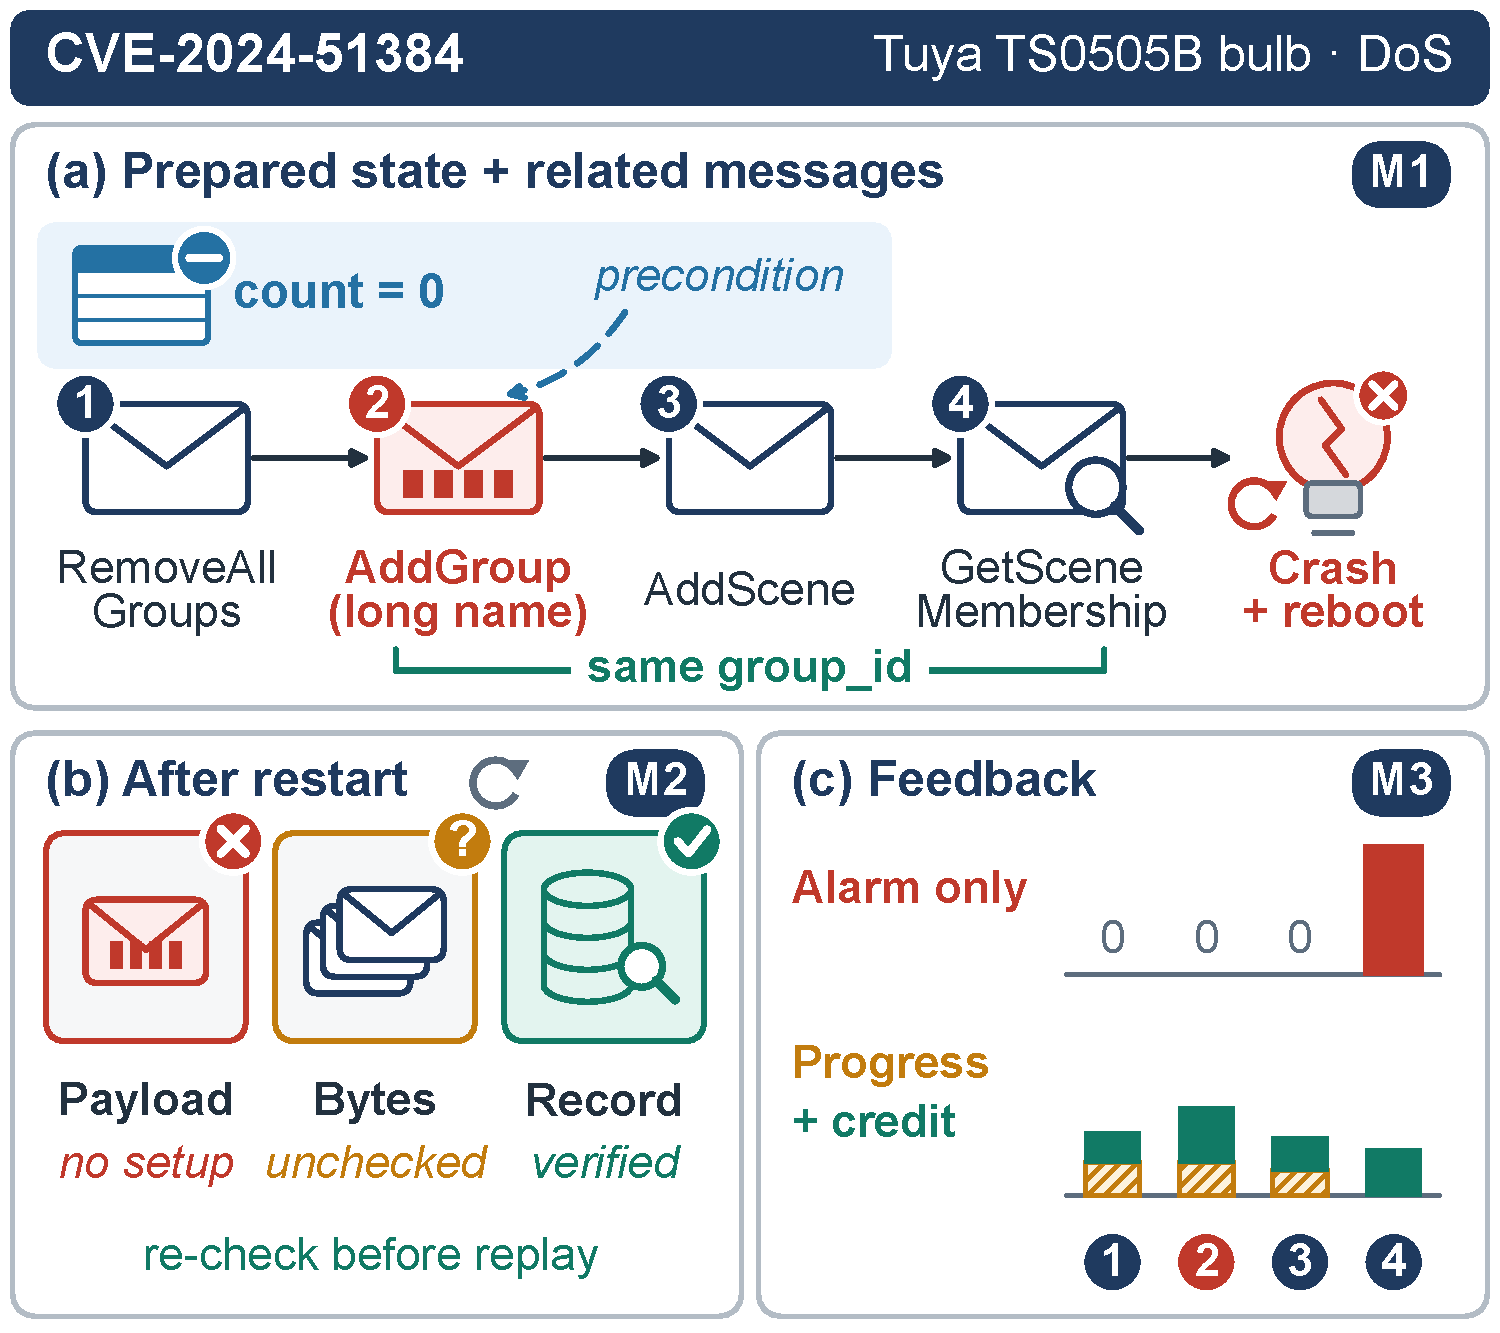
\includegraphics[width=\textwidth]{figure/motivating_example.pdf}
  \caption{Motivating example based on CVE-2024-51384. (a)~An empty group table and correlated Groups/Scenes messages sharing one group identifier precede the crash, motivating joint state-conditioned planning (Motivation~1). (b)~After a restart, reuse must recover and verify these conditions rather than replay a payload or byte trace (Motivation~2). (c)~Normal intermediate responses and delayed detection motivate bounded progress feedback and replay-supported sequence credit (Motivation~3).}
  \label{fig:state-example}
\end{figure*}

\subsection{Motivations}\label{sec:motivations}
\noindent $\bullet$ \textbf{Motivation 1: Agent-guided exploration of combined states.}\label{sec:motivation1}
State-dependent vulnerabilities may require both a particular protocol path and a particular device configuration. Protocol paths arise from ordered message exchanges, whose effects depend on prerequisites and correlations through shared attributes. Single-message mutation omits these interactions, whereas unrestricted sequence enumeration grows rapidly with the number of commands. Capturing only message dependencies can also miss correlated operations that affect the same device state~\cite{zvdetector}.

Device configuration provides the other dimension. Basic and vendor-specific attributes determine how commands execute, while hidden state may become observable only through functional operations. Restricting exploration to directly writable attributes excludes conditions that must instead be established through supported commands~\cite{zvdetector}. Thus, broader protocol exploration alone does not ensure that a test reaches the relevant device configuration, and broader attribute exploration alone does not supply the sequence that exercises it.

The testing target is therefore the \emph{combined space of protocol and device states}, not either space in isolation. In Figure~\ref{fig:state-example}(a), the empty group table supplies a precondition, and correlated Groups/Scenes messages supply the actions preceding fault detection. Enumerating their unrestricted product spends effort on irrelevant or unreachable combinations. An agent-guided black-box fuzzer should instead reason jointly about message relationships and the device conditions relevant to each sequence. LLM-assisted response reasoning and attribute models can inform this selection~\cite{llmif,mgptfuzz}, but a proposed combination is not evidence that the required state has been reached. The motivation is to direct autonomous exploration toward relevant state--sequence combinations, verify their observable execution conditions, and revise subsequent plans from device feedback while preserving intentional malformed inputs.

\noindent $\bullet$ \textbf{Motivation 2: Condition-preserving experience reuse.}\label{sec:motivation2}
Reaching a deep state or reproducing an anomaly can require substantial preparation. Sequence corpora and historical retrieval provide useful experience for later tests~\cite{llmif,malf}. However, a stateful experiment remains useful only when its prerequisites can be recovered. As Figure~\ref{fig:state-example}(b) illustrates, a saved payload omits the required setup, while a complete byte sequence does not establish the device's state after a restart. Firmware changes can further invalidate the recorded assumptions. Reuse must therefore preserve \emph{the conditions that make a sequence applicable}, rather than treating a previously successful sequence as an unconditional seed.

\noindent $\bullet$ \textbf{Motivation 3: Progress-aware long-horizon exploration.}\label{sec:motivation3}
Crashes and security anomalies can remain absent while a sequence is establishing prerequisites or reaching unexplored states. Assigning zero feedback to every normal outcome leaves this progress indistinguishable from repeated traffic. A constant positive reward creates the opposite problem by making familiar loops indefinitely valuable. Moreover, a fault exposed by a later query does not identify which earlier choices supported it. Event severity alone cannot resolve either problem. Exploration needs \emph{bounded progress before an event and evidence-supported sequence contribution after it}, so that a scheduler can compare useful frontiers and promising paths without confusing repeated observations with new discoveries.

\subsection{Challenges and Solutions}\label{sec:challenges}
\noindent \textbf{(CH-1) Executable semantic planning under partial observations.}
The tester observes protocol-level behavior rather than the complete device state. Relevant preconditions may involve hidden attributes or functional commands, and a message relationship inferred from documentation need not be executable on a particular target. Checking every generated packet against a legal schema would also remove intentional malformed tests. The challenge is to establish the required context and distinguish the intended mutation from unrelated construction errors without assuming that an LLM proposal is execution evidence.

\noindent $\bullet$ \textbf{Solution 1: Joint planning with an evidence boundary.}
We represent the protocol route, device setup, and mutation intent as one state-conditioned test. The Mutator combines state-guided message generation with correlated device-state analysis, then uses format-aware mutation to modify the designated message. A Result Checker verifies supported setup and declared intent, while the Monitor checks the reached conditions during execution. This separation preserves negative tests while grounding their context in observations, addressing \textbf{CH-1} (Sections~\ref{sec:state-awareness}, \ref{sec:mutator}, and~\ref{sec:monitor}).

\noindent \textbf{(CH-2) Dependency-preserving reuse with bounded context.}
Keeping an entire campaign in the prompt exceeds the context budget. Keeping only recent exchanges can discard the setup and shared identifiers needed to recover a useful path. Historical observations can also become stale after execution or a restart. The challenge is to retain a compact executable experiment and determine whether its conditions hold now, without using a historical snapshot as evidence of the current state.

\noindent $\bullet$ \textbf{Solution 2: Applicability-aware experimental memory.}
We retain ordered sequences with their target compatibility, initial predicates, and executable setup. Reproduction evidence supports selective promotion to long-term memory. Retrieval supplies a relevant experiment, while fresh observations or verified setup establish its applicability. The Prompt Context Builder injects the current decision context and exposes references for on-demand retrieval. Separating reusable knowledge from runtime state addresses \textbf{CH-2} without requiring the full history in every prompt (Section~\ref{sec:context}).

\noindent \textbf{(CH-3) Informative feedback for sparse and delayed outcomes.}
Progress must remain useful before a fault without rewarding repeated loops indefinitely. After a delayed event, terminal-only credit overlooks earlier choices, whereas uniform backward credit includes unrelated steps and duplicates the event's value. Replay is further constrained by partial observations and ablations that may invalidate the sequence. The challenge is to allocate supported contribution and revise earlier utilities while preserving both the event budget and the number of original trials.

\noindent $\bullet$ \textbf{Solution 3: Decoupled deterministic feedback and contextual scheduling.}
We separate event severity from finite, visit-decayed progress and replay-supported sequence contribution. Confirmation redistributes one event budget across supported steps and revises the utilities of their original experiments without adding trials. Two-level UCB then compares state--message opportunities and mutations within each selected context. A reserved frontier budget and a separate replay budget complement this scheduling. Together, these mechanisms address \textbf{CH-3} by providing bounded exploration signals and conserving delayed-event credit (Sections~\ref{sec:evaluator} and~\ref{sec:mutator}). Replay supports attribution but does not prove firmware-level causality.

\subsection{Threat Model}\label{sec:threat-model}
\parab{Targets and security objectives.}
\system{} tests unmodified IoT devices through their protocol interfaces. Its purpose is to help authorized administrators and manufacturers identify state-dependent failures in firmware and protocol-stack behavior. The relevant security properties include device availability, integrity of protocol-visible state, and enforcement of supported permissions and invariants. A timeout or unexpected response is an observation requiring investigation, not automatically a security vulnerability.

\parab{Access and adversarial inputs.}
The tester controls a compatible gateway or controller and has completed the pairing, commissioning, or authentication needed to communicate with the target. Within this established access, it can issue supported setup commands and send chosen message sequences with intentional field or structural violations. An attacker exploiting a reported fault would need the access required to deliver the same messages. We do not assume that an arbitrary remote attacker can obtain this access, bypass authentication, or change device state through an unavailable operation. Physical pairing and recovery may require an operator and are distinct from autonomous test generation.

\parab{Observations and scope.}
The framework observes protocol responses, traffic, accessible attributes, and device liveness through supported probes. It does not require firmware source code, instrumentation, or internal execution coverage. Hidden state is included only when command-level behavior supports an observation or setup method. Missing evidence remains unknown, and replay requires comparable observable baselines rather than an assumed complete reset. Firmware-only conditions, attacks outside the permitted interface, and failures with no supported observation lie outside the tested abstraction. Protocol documents, responses, and retrieved memories are untrusted inputs to the agents. They cannot authorize tool use beyond the campaign's permitted operations. Experiments are confined to owned or explicitly authorized targets in an isolated testbed.

\section{System Overview}\label{sec:design}
\begin{figure*}[t]
  \centering
  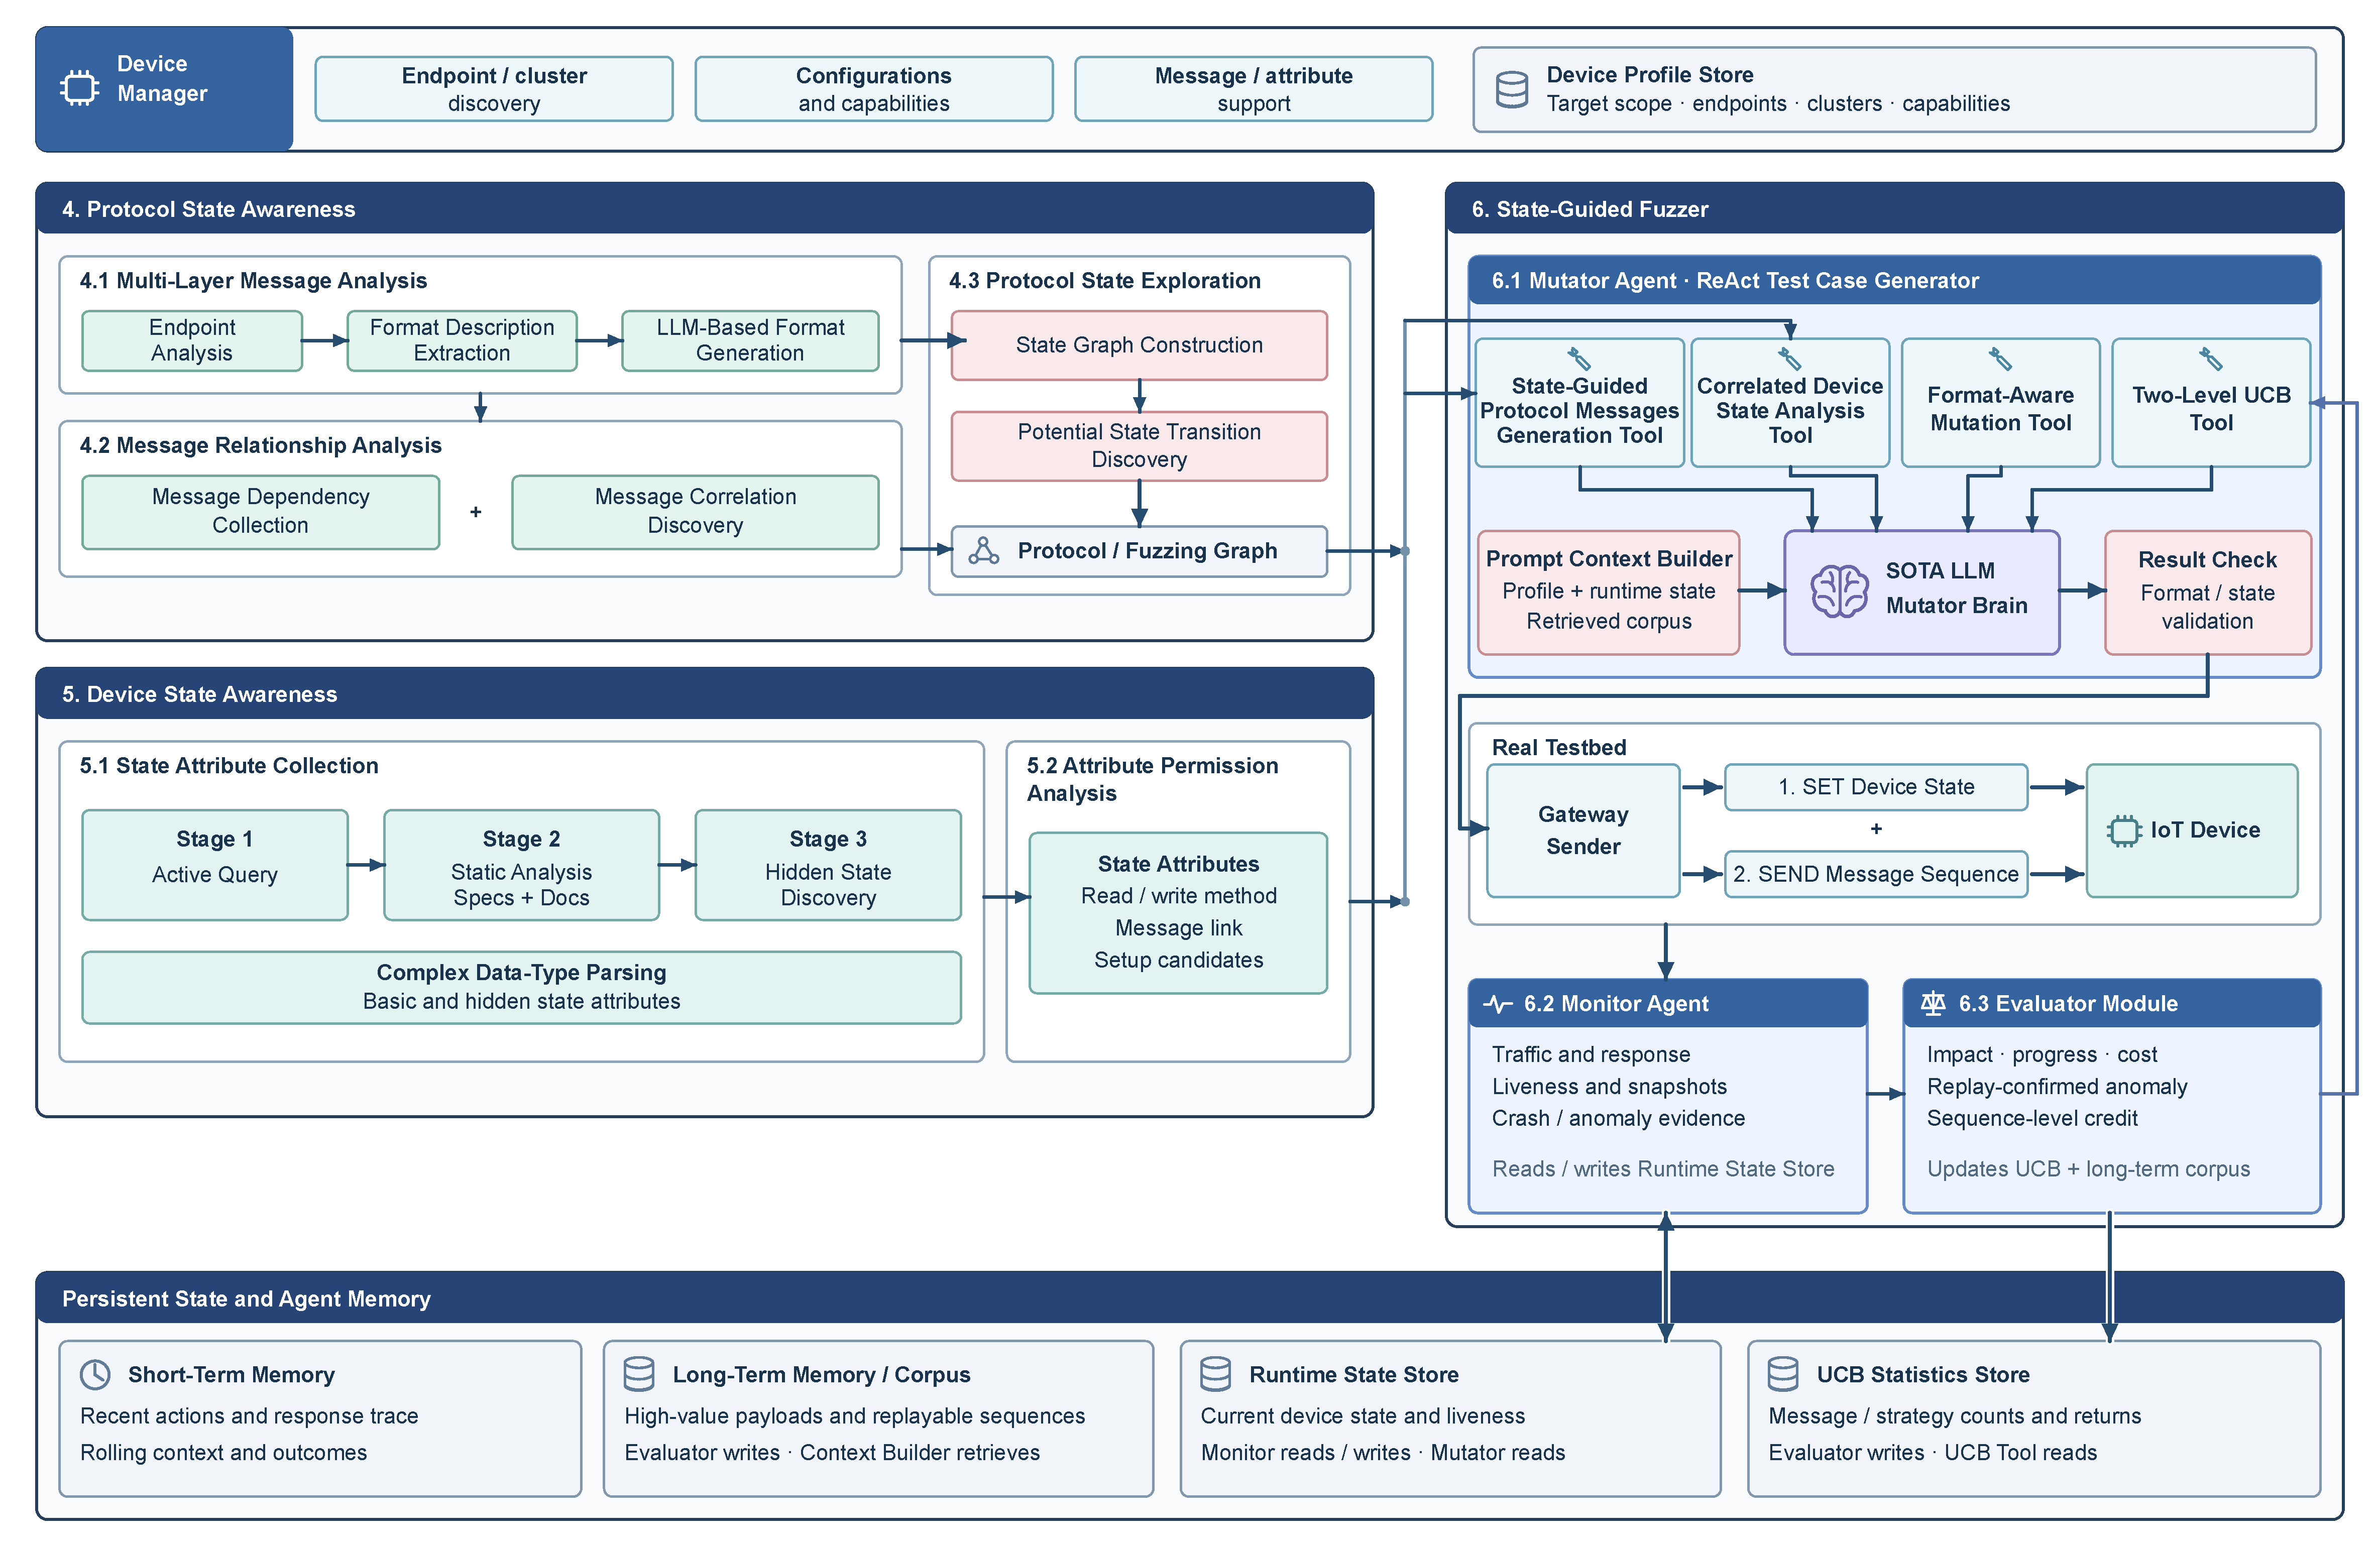
\includegraphics[width=1.0\textwidth]{figure/arch.pdf}
  \caption{Architecture of \system{}. Protocol and device state awareness support agent-guided testing. Conditional memory preserves reusable experiments, and deterministic feedback guides exploration. Numbers identify architecture modules rather than sections of this paper.}
  \label{fig:architecture}
\end{figure*}
Figure~\ref{fig:architecture} shows the modules of \system{}. They share a \emph{state-conditioned test} that binds a mutation and ordered sequence to a compatible target and checked preconditions. The framework separates semantic planning from execution evidence and uses the same experiment as the unit of memory reuse and scheduling feedback.

\noindent $\bullet$ \textbf{Device Manager.}
The Device Manager discovers supported endpoints, clusters, messages, and state-access capabilities. It maintains the Device Profile used to constrain test construction and identify compatible recalled experiments. This capability boundary supports \textbf{CH-1} by excluding unsupported setup operations and \textbf{CH-2} by distinguishing compatible targets from incompatible historical records (Sections~\ref{sec:state-awareness} and~\ref{sec:context}).

\noindent $\bullet$ \textbf{Protocol State Awareness.}
Multi-layer message analysis supplies message formats. Relationship analysis identifies dependencies and correlations, which guide state-graph construction and exploration of candidate transitions. The resulting protocol/fuzzing graph supplies routes and shared-field constraints to the State-Guided Protocol Messages Generation Tool. These relations support \textbf{CH-1} by narrowing planning to meaningful sequences whose reachability can be checked through execution (Section~\ref{sec:state-awareness}).

\noindent $\bullet$ \textbf{Device State Awareness.}
Active queries and document-based analysis collect state attributes and parse their data types. Permission analysis identifies supported observation and state-setting methods, including functional commands for attributes that cannot be written directly. The Correlated Device State Analysis Tool uses these descriptors to select the predicates and setup relevant to a proposed sequence. This module complements protocol reachability with executable device preconditions, addressing the state-preparation aspect of \textbf{CH-1} (Section~\ref{sec:state-awareness}).

\noindent $\bullet$ \textbf{State-Guided Fuzzer.}
The Mutator Agent plans tests through callable analysis, generation, mutation, and UCB tools. The Result Checker verifies construction intent before the Gateway Sender performs setup and sends the sequence to the IoT device. The Monitor Agent checks reached conditions and updates runtime observations, completing the evidence boundary for \textbf{CH-1}. The Evaluator Module separates severity, progress, and sequence contribution, then revises the original utilities consumed by the Two-Level UCB Tool. This feedback loop addresses \textbf{CH-3} while leaving reward construction outside the LLM (Sections~\ref{sec:mutator}--\ref{sec:evaluator}).

\noindent $\bullet$ \textbf{Persistent State and Agent Memory.}
Short-term memory preserves episode continuity, while long-term memory retains condition-preserving experiments for later reuse. The Runtime State Store holds current observations, and the UCB Statistics Store retains trial counts and utilities. The Prompt Context Builder combines current facts with references to relevant experience rather than injecting the full campaign history. This separation addresses \textbf{CH-2} and preserves the distinct evidence used for planning and scheduling (Section~\ref{sec:context}).

The access and observation boundary is defined in Section~\ref{sec:threat-model}. Within that boundary, each proposed test must identify how its prerequisites will be established and how its outcome will be observed. A reset alone is insufficient evidence that persistent state has returned to the required baseline.

\parab{Test definition and scope.}
A test binds an ordered message sequence and its intended mutation to a compatible target profile. It specifies the observable baseline, executable setup, and supported observations or oracle needed to interpret the outcome. The scheduler's pre-state combines a protocol-graph node with the device predicates relevant to the message. Execution evidence must support that pre-state before the intended mutation is treated as tested in its context. Deliberate field violations remain valid testing objectives when transport and setup still make the experiment executable.

The state-conditioned test is also the unit of reuse and scheduling evidence. Setup packets, suffix queries, and verification probes have explicit roles within or alongside the experiment. Their presence in a trace does not make each packet a new mutation trial.

\section{State Awareness}\label{sec:state-awareness}
State awareness combines two complementary views of a test's execution context~\cite{zvdetector}. Protocol awareness supplies message dependencies and routes to a testing context. Device awareness supplies relevant predicates and the operations that can observe or establish them. Their integration exposes \emph{executable conditions} to the Mutator and reusable records, supporting the planning requirements of \textbf{CH-1}.

\parab{Relationship-guided protocol exploration.}
Protocol exploration uses supported endpoints and input/output clusters to delimit the target's message interface. Schemas recovered from protocol libraries, specifications, and available vendor documentation support construction, while missing descriptions remain candidates for target-specific verification. Static semantic analysis and dynamic exchanges reveal dependencies and correlations, including shared fields and affected attributes. Where cross-device communication is available, binding and response probes check proposed out-cluster relationships. These relations support dependency-breaking tests, correlated-message insertion, and individual-transition exploration. For agent planning, the important distinction is between a candidate transition and one supported by execution. The graph retains both without promoting an inferred relation to established reachability.

\parab{Command-accessible device preconditions.}
Device awareness combines active queries with specification, documentation, and message-function analysis. The resulting descriptors cover exposed attributes and state accessible through functional commands, including supported manufacturer-specific or hidden attributes. Each descriptor identifies the attribute's encoding, observation method, and available state-setting operations. This access model is necessary because an attribute marked read-only for \texttt{WriteAttributes} can still change through a functional command. The framework uses these descriptors to express concrete preconditions and setup choices. It includes hidden attributes only when protocol behavior provides a supported means to observe or manipulate them.

\parab{Composing the two views.}
The graph provides a candidate route, and message--attribute relations identify the device predicates that matter along that route. The Mutator can therefore select a relevant state--sequence combination instead of taking the unrestricted product of attribute values and message orders. Subsequent observations refine the relations and validate reached conditions. Incomplete capabilities and unverified LLM proposals remain uncertain, preserving the boundary between semantic guidance and execution evidence.

\section{State-Guided Fuzzer}\label{sec:fuzzer}
The fuzzer carries state-conditioned experiments through execution and reuse. Its design makes three dependencies explicit: planning depends on current conditions, reuse depends on compatibility and retained setup, and scheduling depends on evidence assigned to the original experiment. The following components implement these dependencies without treating an LLM proposal, a historical snapshot, or a repeated alarm as new execution evidence.

\subsection{Condition-Preserving Context and Memory}\label{sec:context}
\parab{Separate present state from reusable knowledge.}
Challenge~2 arises because compatibility, current state, and past behavior answer different questions. The Device Manager identifies what the target supports and which profiles are compatible. The Runtime State Store records current observations, which can become stale after execution or recovery. Long-term memory records behavior under previously tested conditions. Keeping these sources distinct prevents a useful historical sequence from implicitly certifying the current pre-state. Unknown conditions remain unknown until observed or established through verified setup.

Short-term memory maintains continuity within the current episode. The Mutator's recent choices, the Monitor's comparison baseline, and the Evaluator's ordered evidence refer to the same execution history. These views support the next decision without replacing the longer-lived applicability record.

\parab{Retain the conditions that make experience valuable.}
The reuse unit is an experiment rather than an isolated payload. Each high-value record binds the mutation and ordered sequence to its compatible target and initial-state requirements. Executable setup and the reachability prefix preserve how those conditions were obtained, while reproduction evidence records how strongly the outcome is supported. Confirmed graph relations and attribute-access methods accompany the corpus to support later reconstruction. A reduced sequence is retained only as a tested reusable path, without a claim of global minimality.

Promotion to semantic memory depends on evidence and reproducibility, not a high scalar return alone. Repeated executions refine the same record, and incompatible device or firmware assumptions require revalidation. Raw trajectories remain available for audit. In contrast to selective corpus promotion, scheduling statistics retain every valid original decision, including zero-return tests. This distinction keeps reusable knowledge selective without making the scheduler's sample history success-only.

\parab{Retrieve for the current decision.}
Retrieval first restricts experience by target compatibility and then considers the conditions relevant to the candidate message and mutation. A matching record can supply a supported setup and sequence. Broader compatible experience can suggest a hypothesis, but requires further checking before execution. This applicability gate is the distinction between retrieving a similar seed and recovering a meaningful stateful test.

Figure~\ref{fig:conditional-memory} illustrates this distinction. In the running example, the reusable record retains the empty-group requirement and the shared identifiers of the Groups/Scenes operations. If the current group-table condition is unknown, the stored sequence cannot establish that it still holds. The Mutator must obtain a fresh observation or execute and verify the recorded setup before replaying the mutation. A version mismatch likewise requires revalidation instead of transferring the earlier outcome unchanged.

\begin{figure}[t]
  \centering
  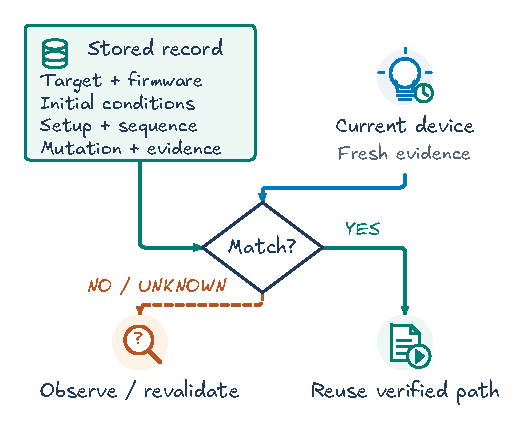
\includegraphics[width=\columnwidth]{figure/conditional_memory_example.pdf}
  \caption{Condition-preserving reuse checks recorded experiments against fresh device evidence. Only compatible conditions permit reuse. Unknown or incompatible conditions require observation or revalidation.}
  \label{fig:conditional-memory}
\end{figure}

The Prompt Context Builder exposes current facts, the testing objective, available resources, and references to relevant experience. Tools retrieve detailed schemas, local graph relations, and replay evidence when the decision requires them. The fixed System Prompt establishes the role and evidence rules, while the dynamic User Prompt carries the changing context. This division limits prompt size without discarding the earlier dependencies that make a recalled sequence useful.

\subsection{Mutator Agent}\label{sec:mutator}
The Mutator addresses Challenge~1 by choosing \emph{where a mutation should be exercised and which conditions must be preserved}. A bounded ReAct loop~\cite{react} supports evidence acquisition and plan revision. Its contribution to the design is the connection between a semantic hypothesis and a checked state-conditioned experiment, rather than the use of an agent loop by itself.

\parab{Couple protocol reachability with device preconditions.}
The \emph{State-Guided Protocol Messages Generation Tool} supplies routes and sequence dependencies, while the \emph{Correlated Device State Analysis Tool} identifies relevant attributes and executable setup operations. The Mutator uses these views to plan a protocol route and its associated device setup together, rather than selecting them independently.

The Mutator distinguishes a \emph{reachability prefix} from the \emph{mutation target}. It preserves a supported prefix and setup when the \emph{Format-Aware Mutation Tool} modifies the designated message. The declared strategy may target field types or boundary values, or introduce semantic or structural violations. A suffix can exercise or observe the state affected by the mutation as part of the same experiment. In the running example, the mutated group name is tested within a Groups/Scenes sequence whose shared identifiers remain consistent. The later query is an observation point, not necessarily the mutated message. Preserving this structure keeps unrelated construction failures from obscuring the behavior under test.

The four tools in Figure~\ref{fig:architecture} expose complementary evidence and choices to the LLM. The agent can inspect relevant attributes, revise a path, or check a recalled sequence before committing to a mutation. They are callable capabilities, not mandatory stages of one pipeline. The \emph{Two-Level UCB Tool} supplies exploration priorities without taking over semantic planning.

\parab{Preserve test intent at the execution boundary.}
The Result Checker checks target compatibility and whether the plan includes supported operations for establishing its stated preconditions. It also verifies that malformed fields correspond to declared testing intentions. Requiring every packet to satisfy a legal schema would suppress precisely the malformed inputs needed for negative testing. Conversely, unintended encoding errors reveal little about the chosen hypothesis. The checker therefore distinguishes declared mutations from accidental construction failures. Observations during execution, not static checking alone, establish that the intended state was reached.

The Gateway Sender executes setup and the ordered sequence while milestone observations check the pre-mutation state. A deviation from the prefix can invalidate both the semantic hypothesis and its scheduled context. The Mutator then replans from the observed state, and feedback belongs to the experiment actually executed. This preserves the meaning of a scheduler trial across multi-message delivery, rather than counting each setup packet as a new mutation decision.

\parab{Separate where to explore from how to mutate.}
A mutation strategy can be productive for one state--message context and ineffective for another. A global strategy mean obscures this dependence by mixing outcomes from different contexts. Enumerating every state--message--strategy--mode combination as an independent arm instead leaves many arms with little evidence. We therefore separate the selection of exploration opportunities from the selection of mutations within each context.

The first level selects a message $m$ under a compatible target profile $p$ and canonical pre-state $s$, represented by arm $(p,s,m)$. Within this context, the second level selects strategy $\mu$ and mutation mode $\nu$, giving arm $(p,s,m,\mu,\nu)$. The mode specifies, for example, whether one or multiple fields are mutated. Capability and reachability constraints restrict the candidates before scoring. Both levels consume the same normalized Evaluator utility $z_d\in[0,1]$ (Section~\ref{sec:evaluator}). For feasible arm $a$ in parent context $h$,
\begin{equation}
U_h(a)=
\begin{cases}
+\infty, & n_a=0,\\
\bar z_a+c\sqrt{\ln(1+N_h)/n_a}, & n_a>0,
\end{cases}
\label{eq:ucb}
\end{equation}
where $n_a$ counts valid original trials of $a$ and $N_h$ counts trials in its parent context. At the first level, the parent is the compatible profile's exploration pool. At the second level, it is the selected state--message arm, ensuring that strategies are compared under the same conditions. Compatible broader experience can guide cold-start suggestions, but does not replace local means or trial counts.

This UCB-inspired tool~\cite{ucb1} balances underexplored opportunities against historical utility. Reward construction and sequence attribution remain the responsibility of the Evaluator. The Mutator may depart from a recommendation when semantic evidence warrants it, in which case feedback is assigned to the actual choice. A reserved frontier budget complements score-based selection. Reproduction receives a separate bounded budget so that verification is not treated as exploration success. The device state evolves, progress bonuses decay, and delayed evidence revises past utility. Because these effects violate the stationary-bandit assumptions, we make no standard UCB1 regret claim.

\subsection{Monitor Agent}\label{sec:monitor}
The Monitor supplies the evidence boundary shared by planning and feedback. A response or attribute change can indicate progress without establishing security impact, while an absent reply can reflect observation failure rather than a crash. The Monitor combines protocol traffic with relevant attribute, liveness, and latency observations under environmental controls. Its output distinguishes observed facts from inferred changes and unresolved conditions, allowing the Mutator to replan and the Evaluator to score the same evidence consistently.

\parab{Maintain a state abstraction suitable for exploration.}
Stable observations relevant to the tested message form a canonical state signature. Volatile metadata, such as sequence numbers and timestamps, do not define new graph states. Reset epochs and arbitrary differences in raw numeric values are likewise excluded from state novelty. Instead, numeric attributes and response classes are represented through protocol-relevant predicates or bounded classes, with raw values retained as evidence. This normalization prevents observation artifacts from being counted as coverage and makes repeated visits comparable.

The Monitor reads the Runtime State Store to establish a baseline and updates it after execution. An update need not indicate a known healthy state: it may record uncertainty or an abnormal condition, including device unavailability or recovery. This bidirectional interaction is distinct from long-term knowledge promotion. Current observations must be reflected immediately even when an anomaly's interpretation is still pending. Otherwise, the next experiment would be planned against obsolete preconditions.

\parab{Distinguish target behavior from observation failure.}
When a response is missing, compatible control probes help distinguish target behavior from a communication failure. Gateway health and radio conditions provide further context, and timing must account for the behavior of sleepy devices. A rejection or timeout after confirmed delivery remains an observed test outcome. A failure to send or capture the test does not. Because probes may themselves affect state, their effects are retained separately from those of the tested message. LLM-assisted summaries can propose an explanation, but the Evaluator receives the underlying evidence and uncertainty rather than an LLM-assigned security score. Replay uses the recorded observations to check whether the baseline is comparable.

\subsection{Evaluator Module}\label{sec:evaluator}
A useful test need not expose a fault, and the message at which a fault becomes visible need not be the only useful choice in its sequence. The Evaluator addresses these two mismatches by separating \emph{event severity}, \emph{observable progress}, and \emph{sequence contribution}. Fixed evidence rules, rather than a learned reward model or an LLM's subjective score, construct the feedback. Determinism applies to a given observation record and configuration, not to the device's execution.

\subsubsection{Multi-Component Deterministic Feedback}
Event severity classifies the observed outcome rather than its value for exploration. Normal behavior receives no event impact, while suspicious symptoms remain provisional until corroborated. Verified semantic violations and persistent abnormalities receive distinct severity levels, with reproducible crashes assigned the highest level in the initial configuration. A semantic violation must be checked against a supported oracle for permissions, invariants, or expected state. A crash classification requires device-level liveness checks and evidence from recovery and replay. A single absent reply is insufficient, and operational failures are distinguished from valid delivered tests.

Progress measures what a test adds to exploration even when no event occurs. For an original decision $d$, let $\mathcal K_d$ contain its validated, distinct progress keys. Stable states and state--message--state transitions represent state and transition coverage, respectively. Additional keys capture state-conditioned response classes, relevant attribute conditions, and meaningful sequence milestones. We define
\begin{equation}
P_d=\min\left(P_{\max},
             \sum_{k\in\mathcal K_d}p_k(n_k)\right),
\label{eq:progress}
\end{equation}
where $n_k$ counts preceding eligible visits. A milestone records completion of a verified dependency or arrival at a deep state or exploration frontier. A new payload or a longer prefix does not qualify on its own. Together with the Monitor's canonicalization, this definition ties progress to observed behavior rather than textual novelty.

Repeated visits can corroborate a path, but should not make a loop indefinitely attractive. We use bounded diminishing confirmation:
\begin{equation}
p_k(n)=
\begin{cases}
p_k(0)/\sqrt{1+n}, & 0\le n<n_{\max},\\
0, & n\ge n_{\max}.
\end{cases}
\label{eq:progress-decay}
\end{equation}
The first visit receives the full bonus, followed by a limited number of visits with decreasing bonuses. The cap matters because square-root decay alone has an unbounded cumulative sum. Visit counts persist across resets. Fixed preparation and verification do not create new progress. These signals provide feedback between normal execution and rare security events without guaranteeing a positive reward at every step.

For decision $d$, the scheduling utility is
\begin{equation}
u_d=D_d+C_dP_d-K_d,
\label{eq:utility}
\end{equation}
where $D_d$ denotes allocated event value and $C_d$ weights progress according to the evidence tier. The tiers distinguish weak observations, corroborated or persistent evidence, and matched reproduction. They are not calibrated probabilities. The bounded cost $K_d$ accounts for execution and recovery. Without an event, $D_d=0$. Severity $I_E$ remains an independent event label rather than being replaced by this scalar. Normal tests can therefore be informative through $P_d$. Repeated alarms do not create independent event value. Confidence and cost affect exploration priorities, not the meaning of the severity class.

\subsubsection{Replay-Supported Sequence Contribution}
Progress alone cannot explain which earlier choices supported a delayed abnormal outcome. For a reproducible event $E$ detected at step $T$, we establish one budget $B_E=C_EI_E$ for its episode. An episode starts at a verified observable baseline. Repeated alarms and escalated labels revise this provisional budget rather than creating independent rewards. At most one event budget, corresponding to the highest supported severity tier, is active before a new episode begins.

Full replay first checks that the baseline and symptom match. Confirmation requires repeated baseline-checked replays, with actual reproduction rates and uncertainty retained. Within the replay budget, ablations remove or simplify candidate preceding steps while preserving an executable sequence and comparable initial state. Let $r_0$ be the reproduction rate of the full sequence and $r_i$ that of a valid ablation. The difference $q_i=\max(0,r_0-r_i)$ measures conditional support for the step's contribution. If an ablation is not executable or fails to match the baseline, its contribution support remains unknown. The same applies to an untested step. Replay provides controlled empirical support, not proof of firmware-level causality.

For each eligible preceding step, its role and state relevance determine how it relates to the test. Replay support and temporal distance then modulate its contribution weight:
\begin{equation}
w_i=\rho_i s_i q_i
     \left[\epsilon+(1-\epsilon)e^{-(T-i)/\tau}\right].
\label{eq:credit-weight}
\end{equation}
Here $\rho_i$ distinguishes setup and transition roles. State relevance $s_i$ is strongest when a verified predicate or dependency links the step to the event. A confirmed state on the replayed path without a direct link receives partial relevance, and other steps receive none. Distance modulates supported contribution rather than replacing it. The floor $\epsilon$ prevents an essential early setup from receiving negligible weight merely because the sequence is long.

When $\sum_{j<T}w_j>0$, allocation is
\begin{equation}
D_i^E=
\begin{cases}
(1-\alpha)B_E, & i=T,\\
\alpha B_Ew_i/\sum_{j<T}w_j, & i<T.
\end{cases}
\label{eq:allocation}
\end{equation}
Otherwise all $B_E$ remains at detection. Consequently,
\begin{equation}
\sum_i D_i^E=B_E.
\label{eq:budget}
\end{equation}
This conservation distinguishes the method from assigning a full terminal reward to every earlier step. Extending the sequence or identifying more contributing steps cannot increase the event's total value. Additional replay can refine the allocation but cannot multiply the budget. Backward contribution therefore redistributes part of the terminal credit rather than adding to it.

Step contributions are mapped to the original decisions that generated them within the same episode. If a suffix or observation probe detects a delayed event, the detection share belongs to the validated test case rather than a new probe arm. Fixed setup and replay prefixes can retain contribution evidence in the corpus but do not reopen historical trials. The resulting $D_d$ expresses experiment-level utility. It does not establish that either the detection step or the selected mutation is the true trigger.

\subsubsection{Count-Preserving Feedback Revision}
Delayed evidence must revise the meaning of an earlier trial rather than increase the number of trials. The Evaluator therefore replaces provisional event allocations after confirmation or rejection and updates each affected arm's accumulated utility by
\begin{equation}
S_a\leftarrow S_a+
       (z_d^{\mathrm{new}}-z_d^{\mathrm{stored}}).
\label{eq:revision}
\end{equation}
The trial counts $n_a$ and $N_h$ remain unchanged. Both scheduling levels receive the same revision, and duplicate or obsolete revisions have no effect. A rejected event loses its provisional impact while preserving any valid progress and cost. Preparation, observation, and replay contribute evidence, not additional scheduler trials.

These update semantics connect long-horizon attribution to two-level selection without double-counting a rare event. They also distinguish statistical reuse from semantic reuse. Every valid decision informs scheduling statistics, including decisions with zero return. Long-term memory instead retains supported relations and reproducible high-value sequences. The next Mutator decision can therefore recover the conditions for reaching a useful behavior together with evidence about the exploration choices that supported it.

\parab{Worked allocation.}
Figure~\ref{fig:sequence-credit} gives an arithmetic illustration. Let a confirmed event have budget $B_E=15$ and let $\alpha=0.4$. Suppose two preceding steps have supported weights in the ratio $1:2$, while an unrelated step has zero support. The detection step retains $9$ units, and the preceding steps receive $2$ and $4$ units. Total event value remains $15$. These step shares are then mapped to their original experiments. If a later probe reveals the event, its detection share revises the validated test's utility rather than creating a new probe trial. A normal experiment can independently receive bounded progress without inheriting this event budget.

\begin{figure}[t]
  \centering
  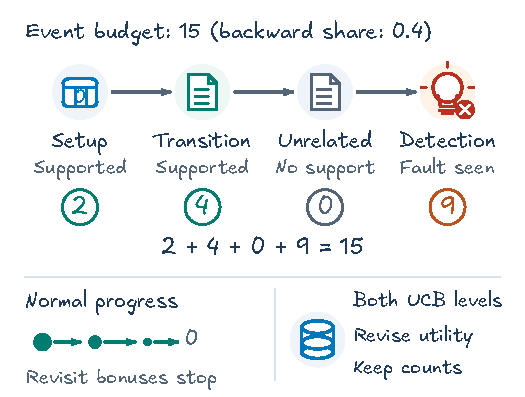
\includegraphics[width=\columnwidth]{figure/sequence_credit_example.pdf}
  \caption{Allocation of one event budget across replay-supported steps. The shares sum to 15, with no credit for the unsupported step. Normal progress bonuses diminish and stop. Both UCB levels revise original utilities without adding trials.}
  \label{fig:sequence-credit}
\end{figure}

\parab{Bounded configuration.}
Bounds on event value, progress, and cost define a fixed utility range for UCB normalization. Shared setup and recovery costs are charged once per original experiment. Changing the score scale requires recomputation or a new scheduling epoch. Finite progress and conserved event value preserve the feedback semantics independently of the chosen numerical settings. Section~\ref{sec:setup} specifies the initial configuration and normalization.

\section{Evaluation}\label{sec:evaluation}
We evaluate state awareness, vulnerability detection, and the effectiveness and cost of the agent mechanisms through the following five research questions.\label{sec:rq}

\noindent $\bullet$ \textbf{\rq{1}: Protocol state awareness.} How accurately can the framework recover message formats, dependencies, and correlations?

\noindent $\bullet$ \textbf{\rq{2}: Device state awareness.} How effectively can it collect attributes, identify their access methods, and parse complex types?

\noindent $\bullet$ \textbf{\rq{3}: Vulnerability detection.} Can it reproduce state-dependent vulnerabilities and discover additional faults?

\noindent $\bullet$ \textbf{\rq{4}: Planning and memory.} Do verified preconditions and conditional memory improve test execution and path recovery?

\noindent $\bullet$ \textbf{\rq{5}: Feedback, scheduling, and cost.} How do long-horizon feedback and two-level UCB affect exploration and operational cost?

\subsection{Experimental Setup}\label{sec:setup}
\parab{Testbed.}
Table~\ref{tab:reference-devices} summarizes the 14 IoT devices selected for our experiments, covering seven device types and two protocols: Zigbee and Z-Wave. These devices come from eight vendors: Aqara, Tuya, Sengled, Tuya OMEG, Third Reality, Aeotec, Zooz, and NewOne.

\begin{table}[t]
\centering
\caption{14 Zigbee and Z-Wave devices used in our testbed.}\label{tab:reference-devices}
\small
\renewcommand{\arraystretch}{1.15}
\begin{tabularx}{\columnwidth}{@{}r l l >{\raggedright\arraybackslash}X@{}}
\toprule
\textbf{ID} & \textbf{Type} & \textbf{Vendor} & \textbf{Model} \\
\midrule
\rowcolor{zigbeebg}[0pt][0pt]\multicolumn{4}{@{}l@{}}{\textbf{Zigbee}} \\
1 & Plug & Aqara & lumi.plug \\
2 & Switch & Tuya & SM0004 \\
3 & Plug & Tuya & TS011F \\
4 & Bulb & Tuya & TS0505B \\
5 & Switch & Sengled & E1E-G7F \\
6 & Bulb & Sengled & E11-N1EAW \\
7 & Strip & Sengled & E1G-G8E \\
8 & Valve & Tuya OMEG & TS0049 \\
9 & Bulb & Third Reality & 3RCB01057Z \\
10 & Plug & Third Reality & 3RSP02028BZ \\
\rowcolor{zwavebg}[0pt][0pt]\multicolumn{4}{@{}l@{}}{\textbf{Z-Wave}} \\
11 & Remote & Aeotec & WallMote 7 (ZWA022-A) \\
12 & Switch & Zooz & ZEN76 800LR \\
13 & Plug & NewOne & N4011 800S \\
14 & Dimmer & Zooz & ZEN77 800LR \\
\bottomrule
\end{tabularx}
\end{table}

For Zigbee, we use the SONOFF Zigbee 3.0 USB Dongle Plus (DongleP) and Nortek GoControl QuickStick HUSBZB-1 (HUBZ) as USB-connected gateways, with HUBZ integrated into Home Assistant via Zigbee Home Automation (ZHA). A separate CC2531 USB dongle connected to a Windows 11 host running TiWsPc captures Zigbee traffic~\cite{zvdetector}. For Z-Wave, a Zooz 800 Series Z-Wave Long Range S2 USB Stick (ZST39 LR) serves as the gateway for sending messages and receiving device responses~\cite{zst39manual}. A separate Silicon Labs ACC-UZB3-S USB sniffer works with the Z-Wave Zniffer application to capture Z-Wave traffic~\cite{uzbmanual}.

\parab{Implementation configuration.}\label{sec:implementation}
Agent and all experiments ran on Ubuntu 20.04 virtual machines with a 2.6~GHz six-core Intel Core i7 and 16~GB of memory. Home Assistant 2024.4.2 hosted the ZHA network. DeepSeek-V4.1-Flash serves as the state-perception module and as the LLM underlying all agents, supporting a context window of up to 1M tokens. We use LangGraph ~\cite{langgraph} for agent orchestration and custom ReAct loops~\cite{react}, with LangChain ~\cite{langchain} providing the model and tool interfaces; model API errors are retried at most twice additionally. The Mutator is limited to at most 13 model calls and 10 tool calls per conversation, while the Monitor defaults to a maximum of 8 rounds. Memory is maintained as files that record the target device's profile for each round, the results of each agent, and reusable experience.

% gpt-5.6-sol作为状态感知模块，以及各个Agent使用的llm，且支持1M的上下文窗口大小。我们采用LangGraph进行agent的编排和自定义ReAct循环，并使用langchain来提供模型与工具接口，模型API错误最多额外重试2次。Mutator每次对话限制最多13轮模型调用，10次工具调用；Monitor默认最多8轮。记忆以文件的形式记录每一轮目标设备的profile，各个Agent的结果以及可复用经验。

\parab{Feedback and scheduling configuration.}
Table~\ref{tab:feedback} lists the initial parameters. Progress rewards decay over three eligible visits, and one in five dispatch slots is reserved for a feasible frontier. Event confirmation requires at least two of three matched replays. Utilities satisfy $u_d\in[-1,18]$ and are normalized as $z_d=(u_d+1)/19$.

% 导言区新增（紧跟 zigbeebg/zwavebg 之后）
\definecolor{groupbg}{RGB}{238,238,245}  % light neutral band for group rows

\begin{table}[!t]
\centering
\caption{Initial feedback and scheduling configuration.}\label{tab:feedback}
\small
\setlength{\tabcolsep}{4pt}
\renewcommand{\arraystretch}{1.15}
\begin{tabularx}{\columnwidth}{@{}l >{\raggedright\arraybackslash}X@{}}
\toprule
\textbf{Parameter} & \textbf{Initial value} \\
\midrule
\rowcolor{groupbg}[0pt][0pt]\multicolumn{2}{@{}l@{}}{\textbf{Event feedback}} \\
\addlinespace[2pt]
Normal outcome & $0$ \\
Suspicious symptom & $2$ (provisional) \\
Verified semantic violation & $6$ \\
Persistent abnormality & $10$ \\
Reproducible crash & $15$ \\
Evidence weight $C$ & Weak $0.3$, corroborated $0.7$, replay-matched $1$ \\
\rowcolor{groupbg}[0pt][0pt]\multicolumn{2}{@{}l@{}}{\textbf{Progress and cost}} \\
\addlinespace[2pt]
First-visit bonuses & State $1.5$, transition $1$, response $0.5$, attribute $0.3$, sequence $0.5$ \\
Frontier bonus cap & $0.5$ \\
Progress cap $P_{\max}$ & $3$ per experiment \\
Rewarded visits $n_{\max}$ & First $3$ eligible visits \\
Extra retry penalty & $0.1$ per retry, cap $0.3$ \\
Latency $>2\times$ baseline & $0.2$ \\
Reset or recovery penalty & $0.5$ \\
Total cost cap & $1$ \\
\rowcolor{groupbg}[0pt][0pt]\multicolumn{2}{@{}l@{}}{\textbf{Sequence contribution}} \\
\addlinespace[2pt]
Backward fraction $\alpha$ & $0.4$ \\
Role weight $\rho_i$ & Setup $0.5$, transition $0.75$ \\
State relevance $s_i$ & Verified link $1$, on-path state $0.5$, otherwise $0$ \\
Temporal weighting & Floor $\epsilon=0.1$, scale $\tau=8$ steps \\
\rowcolor{groupbg}[0pt][0pt]\multicolumn{2}{@{}l@{}}{\textbf{Verification and scheduling}} \\
\addlinespace[2pt]
Replay confirmation & At least $2$ of $3$ matched replays \\
UCB exploration $c$ & $\sqrt{2}$ \\
Frontier reservation & $1$ in $5$ available dispatch slots \\
\bottomrule
\end{tabularx}
\end{table}

\parab{Baselines.}
ZVDetector~\cite{zvdetector} is our previously proposed combined-state method. Auto-VD retains ZVDetector's ability to perceive both types of states and extends it in terms of vulnerability detection capability and discovery efficiency. We therefore compare Auto-VD with ZVDetector from these two perspectives (\rq{3}, \rq{5}).
\textcolor{red}{\textbf{B1:}} LLMIF~\cite{llmif} has been proven effective in message format generation and relationship discovery \textbf{(\rq{1})}. We construct the same LLM prompts used in LLMIF. We also integrate LLMIF with the initial message mutation strategy of Auto-VD to perform protocol state fuzzing. \textbf{(\rq{3})}.
\textcolor{red}{\textbf{B2:}} Another protocol state fuzzing method proposed by Fiter\u{a}u-Bro\c{s}tean et al.~\cite{fiterau2020analysis,fiterau2023automata}, which follows the DTLS-Fuzzer framework~\cite{fiterau2023automata}. We implement their model learning using LearnLib~\cite{learnlib} to collect message dependencies \textbf{(\rq{1})}, and change the fuzzing method of TLS-Attacker~\cite{tlsattacker} to adapt to Zigbee and Z-Wave \textbf{(\rq{3})}, as its mutation strategy is tailored to the TLS characteristics. Here, B2 uses the results extracted by AutoVD as the registry for protocol message matching.
\textcolor{red}{\textbf{B3:}} Beehive~\cite{wang2022don} is effective in vulnerability discovery using single protocol message fuzzing \textbf{(\rq{3})}. We implement its mutation method and perform semantic-aware fuzzing based on the message formats extracted by Auto-VD.
\textcolor{red}{\textbf{B4:}} HubFuzzer~\cite{ma2023no} is proved to be effective in attribute collection \textbf{(\rq{2})} and combined state fuzzing \textbf{(\rq{3})}. We reuse the prototype from that comparison~\cite{zvdetector}.

% ZVDetector~\cite{zvdetector} is the primary combined-state baseline and anchors the full-system comparison (RQ3, RQ5). \textbf{B1:} LLMIF~\cite{llmif} has been proven effective in message format generation and relationship discovery \textbf{(RQ1)}. We construct the same LLM prompts used in LLMIF. We also integrate LLMIF with our message mutation strategy to perform protocol state fuzzing \textbf{(RQ3)}. \textbf{B2:} Another protocol state fuzzing method proposed by Fiter\u{a}u-Bro\c{s}tean et al.~\cite{fiterau2020analysis,fiterau2023automata}, which follows the DTLS-Fuzzer framework~\cite{fiterau2023automata}. We implement their model learning using LearnLib~\cite{learnlib} to collect message dependencies \textbf{(RQ1)}, and change the fuzzing method of TLS-Attacker~\cite{tlsattacker} to adapt to Zigbee and Z-Wave \textbf{(RQ3)}, as its mutation strategy is tailored to the TLS characteristics. \textbf{B3:} Beehive~\cite{wang2022don} is effective in vulnerability discovery using single protocol message fuzzing \textbf{(RQ3)}. We implement its mutation method and perform semantic-aware fuzzing based on our extracted message formats. \textbf{B4:} HubFuzzer~\cite{ma2023no} is proved to be effective in attribute collection \textbf{(RQ2)} and combined state fuzzing \textbf{(RQ3)}. We reuse the prototype from that comparison~\cite{zvdetector}.

\parab{Budgets and measurements.} 
The planned budget is 24 hours with ten independent runs per device and variant, using randomized method order and comparable initial states. Elapsed time includes setup, model calls, delivery, monitoring, replay, and recovery.
% \todo{Record actual hardware, firmware, plug identifiers, inclusion modes, runtime settings, and completed runs.}

\subsection{State Awareness Effectiveness}\label{sec:overall-results}

\begin{table}[t]
\centering
\caption{Comparison of protocol state-awareness performance, measured by the number of correctly generated Zigbee and Z-Wave message formats and inter-message relations.}
\label{tab:reference-protocol}
\small

\begin{tabularx}{\columnwidth}{@{}X r r r@{}}
\toprule
\rowcolor{zigbeebg}[0pt][0pt]
\multicolumn{4}{@{}l@{}}{\textbf{Zigbee}} \\
Category & B2 & B1 & AutoVD \\
\midrule
ZCL formats & -- & 220 & 382 \\
ZDP formats & -- & -- & 85 \\
APS command / ACK & -- & -- & 10 / 1 \\
NWK command & -- & -- & 13 \\
MAC command / ACK & -- & -- & 9 / 1 \\
\textbf{Total formats} & -- & \textbf{220} & \textbf{501} \\
\midrule
Dependencies & 325 & -- & 366 \\
Basic + Hidden Correlations & -- & \textbf{417} & \textbf{3,150} \\
Cross-device  Correlations & -- & 99 & 612 \\
\bottomrule
\end{tabularx}

\smallskip

\begin{tabularx}{\columnwidth}{@{}X r r r@{}}
\toprule
\rowcolor{zwavebg}[0pt][0pt]
\multicolumn{4}{@{}l@{}}{\textbf{Z-Wave}} \\
Category & B2 & B1 & \system{} \\
\midrule
Application & -- & 31 & 32 \\
Management & -- & 57 & 60 \\
Transport-Encapsulation & -- & 21 & 21 \\
Network-Protocol & -- & 6 & 6 \\
\textbf{Total formats} & \textbf{--} & \textbf{115} & \textbf{119} \\
\midrule
Dependencies & 65 & -- & 92 \\
Basic + Hidden Correlations & -- & 53 & 337 \\
Cross-device correlations & -- & 1 & 29 \\
\bottomrule
\end{tabularx}
\end{table}

\subsubsection{Protocol State Awareness (\rq{1})}
\parab{Message Format Generation Effect.}
Table~\ref{tab:reference-protocol} compares message-format coverage and inter-message relationships for Zigbee and Z-Wave. For Zigbee, AutoVD produces 501 formats, compared with 220 for B1~\cite{zvdetector}. For Z-Wave, AutoVD generates 119 command formats, while B1 produces parser-accepted format descriptions for 115 commands. B2 uses an input catalogue of command formats for model learning, so it does not independently extract message layouts. Each generated message format is validated against real network traffic.

% 相比之下，B1只针对通用ZCL消息格式进行提取。因此，AutoVD可以覆盖更广的协议层和消息类型。

\textbf{For Zigbee}, AutoVD generates 382 Zigbee Cluster Library (ZCL) formats: 279 non-manufacturer-specific cluster messages, 83 manufacturer-specific messages, and 20 general messages. We validate every generated format against captured traffic. On non-manufacturer-specific ZCL messages, B1 achieves 78.85\% accuracy, while AutoVD generates all formats correctly. AutoVD also covers manufacturer-specific messages, which account for a substantial share of real device behavior. \textbf{For Z-Wave}, AutoVD successfully generates 119 command formats across 20 command classes (CCs), covering functions such as switch control and scene configuration. B1 also generates the same number of message formats, but four of them fail parsing validation because the messages contain syntax errors. This is because B1 lacks a format correction mechanism and generates formats through only a single round of LLM analysis, with no repair or regeneration after a parsing failure.

% AutoVD成功生成了20个命令类(CC) 的119种命令格式，涵盖开关控制，场景配置等功能。B1也成功生成了相同数量的消息格式，但是其中4个未能通过解析验证，消息存在语法错误。这是由于B1缺失格式纠错，且仅通过一轮LLM分析生成，解析失败后没有修复或重新生成。

% 对于Zigbee，AutoVD成功发现了366个dependencies，其中包括156个请求响应依赖，以及3150correlations:。

% 相较于B1只发现了417个basic correlations，AutoVD覆盖了更广的协议消息，并且增强了两条消息关联判断的证据，不局限于严格写-读顺序，检查了更多影响共同属性的情况。此外，AutoBD结合字段语义、消息功能和设备属性信息，能够识别格式中没有直接体现的hidden correlations，例如配置命令改变定时行为，进而影响开关命令的执行效果。而对于dependencies的挖掘，AutoVD 结合协议响应与设备属性反馈，能够区分响应相同但实际状态不同的执行上下文，并通过流量分析直接识别请求—响应及 ACK 等因果依赖。相比之下，B2 的状态机学习受输出抽象粒度和有限查询预算影响，可能遗漏细粒度状态及较长前置序列中的依赖；AutoVD 的关系与属性引导探索有助于覆盖这些情况。


\parab{Message relationships.} For Zigbee, Table~\ref{tab:reference-protocol} captures 366 dependencies and 3,150 correlations: 904 basic and 2,246 hidden. The 612 cross-device correlations form a subset of this total. In contrast, B1 discovers only 417 basic correlations. For Z-Wave, AutoVD identifies 92 dependencies and 337 correlations, including 158 basic correlations and 179 hidden correlations. Besides, AutoVD discovers 29 cross-device correlations involving associations between remote controller commands and switch/dimmer commands. 

By contrast, B1 identifies only 53 of the basic correlations. This is because AutoVD covers a broader range of protocol messages and reinforces the evidence for judging correlations between message pairs. AutoVD is not confined to strict write–read ordering. Instead, it examines a wider variety of scenarios in which messages affect shared attributes. Moreover, AutoVD incorporates field semantics, message functionality, and device attribute information. This enables it to identify hidden correlations that are not directly manifested in the message format. A representative example is a configuration command that alters timing behavior and thereby compromises the outcome of a subsequent switch command. For dependency mining, AutoVD leverages protocol responses in conjunction with device attribute feedback. This allows it to distinguish execution contexts that yield identical responses yet differ in actual state. It also pinpoints causal dependencies, such as request–response and ACK relations, directly through traffic analysis. B2, by contrast, learns its state machine under coarse output abstraction and a limited query budget, and therefore overlook fine-grained states and dependencies embedded in longer prerequisite sequences. Consequently, B2 discovers 41 and 27 fewer dependencies than AutoVD on Zigbee and Z-Wave, respectively.

% 因此，B2在Zigbee和Z-Wave上比AutoBD少发现了41个和27个dependencies。

% 对于Z-Wave， AutoVD 成功识别出 337 个correlations，其中包括 158 个basic correlations和 179 个hidden correlations。此外，AutoVD发现 29 个跨设备correlations，涉及遥控器与开关/调光器命令之间的关联。而B1只发现了其中53个basic correlations。

% 和Zigbee发现更多关联关系的原因，

\begin{table}[!t]
\centering
\caption{Device endpoint information coverage results. Clusters and Cmds. count Zigbee clusters and commands; CC and CC Cmds. count Z-Wave command classes and command formats. Numbers in parentheses indicate hidden attributes.}\label{tab:state-coverage}
\small
\setlength{\tabcolsep}{3pt}
\begin{tabularx}{\columnwidth}{@{}r *{6}{>{\centering\arraybackslash}X}@{}}
\toprule
\rowcolor{zigbeebg}[0pt][0pt]\multicolumn{7}{@{}l@{}}{\textbf{Zigbee Devices}} \\
 & \multicolumn{3}{c}{Auto-VD} & \multicolumn{3}{c}{HubFuzzer (B4)} \\
\cmidrule(lr){2-4}\cmidrule(lr){5-7}
ID & Clusters & Attrs. & Cmds. & Clusters & Attrs. & Cmds. \\ \midrule
1 & 16 & 237 & 60 & 11 & 166 & 40 \\
2 & 8 & 73 & 64 & 5 & 44 & 40 \\
3 & 13 & 357 & 102 & 9 & 320 & 74 \\
4 & 10 & 166 & 129 & 8 & 114 & 86 \\
5 & 10 & 72 & 57 & 5 & 42 & 26 \\
6 & 9 & 117 & 58 & 8 & 99 & 48 \\
7 & 9 & 117 & 58 & 8 & 99 & 48 \\
8 & 10 & 79 & 58 & 5 & 44 & 40 \\
9 & 8 & 137 & 79 & 7 & 114 & 68 \\
10 & 10 & 339 & 85 & 8 & 308 & 74 \\ \bottomrule
\end{tabularx}

\smallskip
\begin{tabular*}{\columnwidth}{@{\extracolsep{\fill}}rcccccc@{}}
\toprule
\rowcolor{zwavebg}[0pt][0pt]\multicolumn{7}{@{}l@{}}{\textbf{Z-Wave Devices}} \\
 & \multicolumn{3}{c}{Auto-VD} & \multicolumn{3}{c}{HubFuzzer (B4)} \\
\cmidrule(lr){2-4}\cmidrule(lr){5-7}
ID & CC & CC Cmds. & Attrs. & CC & CC Cmds. & Attrs. \\ \midrule
11 & 17 & 106 & 47 (20) & 12 & 74 & 18 \\
12 & 17 & 103 & 46 (20) & 13 & 78 & 19 \\
13 & 14 & 67 & 27 (17) & 11 & 49 & 7 \\
14 & 17 & 107 & 60 (22) & 13 & 81 & 27 \\ \midrule
\textbf{Total} & 65 & 383 & \textbf{180 (79)} & 49 & 282 & 71 \\ \bottomrule
\end{tabular*}
\end{table}

\subsubsection{Device State Awareness (\rq{2})}
Table~\ref{tab:state-coverage} shows that \system{} identifies more endpoint information than HubFuzzer (B4) on all 14 devices. Aggregated over the ten Zigbee devices, \system{} collects 39.2\% more clusters, 25.5\% more attributes, and 37.9\% more commands. HubFuzzer extracts non-manufacturer-specific clusters from setup messages and omits endpoint out-clusters. By combining active probing with specification and vendor-document analysis, \system{} additionally collects 11 manufacturer-specific clusters, 18 out-clusters, and 44 manufacturer-specific attributes. These include 16 manufacturer-specific attributes within standard clusters, which require analysis beyond the standard attribute catalog.

Across the four Z-Wave devices, \system{} covers 32.7\% more command classes and 35.8\% more command formats than B4. Its expanded state inventory contains 180 attributes, compared with 71 for B4 (153.5\% more). Vendor documentation and message-semantic analysis extend the inventory beyond configuration parameters to state retained across protocol exchanges, which the predefined function and attribute catalog of B4 does not capture. For the NewOne N4011 800S, analysis uses the 14 documented command classes and a conservative subset of 67 formats, excluding later-version features where the manual does not specify a version.

\parab{Hidden attributes and access methods.}
On the Zigbee devices, \system{} validates 116 hidden attributes and identifies 64 message-readable, 67 message-reportable, and 295 message-writable attributes, with overlap between categories~\cite{zvdetector}. Message-semantic analysis enables \system{} to infer state and access methods beyond the predefined attributes and known setter mappings used by B4. In particular, functional commands provide additional ways to observe or modify state, including attributes marked read-only for \texttt{WriteAttributes}. Validation rejects 21.05\% of hidden-attribute candidates and 15.98\% of permission candidates, filtering unsupported LLM proposals~\cite{zvdetector}. 

For Z-Wave, DeepSeek-assisted message analysis identifies 79 additional attributes absent from the known inventories: 20, 20, 17, and 22 for devices 11--14, respectively. On the N4011 800S, the 17 additions capture segment reassembly, saved power-test results, security and supervision sessions, and firmware-update state, increasing Attrs. from 10 to 27~\cite{zwaveapp2024b}. These counts are source-grounded inferences for documented capabilities in classic mesh operation, excluding unconfirmed optional functions; together with the 116 validated Zigbee hidden attributes, they yield a combined inventory of 195 hidden attributes.

\parab{Complex data types.}
For Zigbee, \system{} parses 107 objects containing 120 fields and attributes across six complex types, compared with 25 objects for B4~\cite{zvdetector}. B4 fails to parse complex types in manufacturer-specific objects and some standard objects, such as those using \texttt{StructClass} or \texttt{LVList}. \system{} combines recursive type analysis of protocol libraries with field-level extraction from vendor documentation, recovering structured and variable-length layouts that B4 misses. For Z-Wave, AutoVD supports version-aware parsing, which covers association lists, endpoint-qualified destinations and Configuration bulk records, extending state observation to compound values~\cite{zwavexml}.

\parab{Awareness acquisition cost.}
Format generation for 119 non-ZCL messages took 22.81 minutes. Correlation analysis took 17.2 hours for 6,976 batches and 136,082 message pairs. Hidden-attribute analysis took 9.4 and 35.1 minutes at the device and larger scales, respectively. Permission analysis took 6.19 and 27.77 hours~\cite{zvdetector}. Cost accounting separates awareness acquisition from agent execution. For Z-Wave, acquisition comprises profile construction, command-format resolution, state-access checks, and relationship analysis.

\subsection{Vulnerability Detection Performance}\label{sec:ablation}

\subsubsection{Found Vulnerabilities and Case Study}
\parab{Vulnerability findings (\rq{3}).}
Table~\ref{tab:reference-vulnerabilities} organizes \system{}'s detection inventory into three categories: reproduced ZVDetector vulnerabilities, new found Zigbee vulnerabilities, and new Z-Wave candidates. The reference-reproduction group covers 25 vulnerabilities across seven devices, comprising 18 crashes and seven abnormal-state findings~\cite{zvdetector}. The additional groups contain eight Zigbee vulnerabilities across five devices and four Z-Wave candidates across four devices. They concern timer cancellation, scene isolation and lifecycle management, association consistency, and configuration-dependent control. 


\begin{table}[!t]
\centering
\caption{\system{} detection inventory: reproduced reference vulnerabilities~\cite{zvdetector} and new Zigbee and Z-Wave candidates. New entries and their effects await validation.}\label{tab:reference-vulnerabilities}
\footnotesize
\setlength{\tabcolsep}{3pt}
\renewcommand{\arraystretch}{1.12}
\begin{tabularx}{\columnwidth}{@{}c >{\raggedright\arraybackslash}X >{\centering\arraybackslash}p{0.15\columnwidth} c@{}}
\toprule
\multicolumn{4}{@{}l@{}}{\textbf{Reproduced ZVDetector Vulnerabilities}} \\
\midrule
\multicolumn{3}{@{}l}{IDs 1--7: 18 crashes, 7 abnormal-state findings} & \textbf{25} \\
\midrule
\multicolumn{4}{@{}l@{}}{\textbf{New Zigbee Vulnerability Candidates}} \\
\midrule
\textbf{ID} & \textbf{Triggering messages and conditions} & \textbf{Effect} & \textbf{Count} \\
\midrule
3 & \emph{OnWithTimedOff/WriteAttributes}: zero on-time during an active timer.
  & Abnormal state & 1 \\
\cmidrule(lr){2-4}
4 & \emph{StoreScene, RemoveAllGroups, AddGroup, RecallScene}: reuse the removed group ID.
  & Abnormal state & 1 \\
\cmidrule(lr){2-4}
6 & \emph{MoveToLevel/Stop}: stop during a transition.\newline
    \emph{StoreScene/RecallScene}: same scene ID in different groups.
  & Abnormal state (2) & 2 \\
\cmidrule(lr){2-4}
7 & \emph{StoreScene}: 16 stores with the same IDs.\newline
    \emph{RecallScene/RemoveScene/AddScene}: reuse IDs during a transition.
  & Abnormal state (2) & 2 \\
\cmidrule(lr){2-4}
9 & \emph{MoveToHueAnd\-Saturation, MoveTo\-ColorTemperature}: switch modes during a transition.\newline
    \emph{AddScene/RecallScene}: truncated extension data when updating a scene.
  & Abnormal state (2) & 2 \\
\midrule
\multicolumn{3}{r}{\textbf{New Zigbee subtotal}} & \textbf{8} \\
\midrule
\multicolumn{4}{@{}l@{}}{\textbf{New Z-Wave Vulnerability Candidates}} \\
\midrule
\textbf{ID} & \textbf{Triggering messages and conditions} & \textbf{Effect} & \textbf{Count} \\
\midrule
11 & \emph{Association Set/Remove, Multi Channel Association Set/Get}\newline
     Truncated endpoint tuple after membership changes while awake.
   & Abnormal state & 1 \\
\cmidrule(lr){2-4}
12 & \emph{Configuration Set/Get, Switch Binary Set}\newline
     Attempt switching with local and Z-Wave relay control disabled.
   & Abnormal state & 1\\
\cmidrule(lr){2-4}
13 & \emph{Configuration Set/Get, Switch Binary Get}\newline
     For a supported timer, truncate the value but retain its declared size.
   & Abnormal state & 1\\
\cmidrule(lr){2-4}
14 & \emph{Switch Multilevel Set, Start/Stop Level Change, Get}\newline
     Interleaved dimming near brightness limits during a transition.
   & Abnormal state & 1 \\
\midrule
\multicolumn{3}{r}{\textbf{New Z-Wave subtotal}} & \textbf{4} \\
\midrule
\multicolumn{3}{r}{\textbf{Total}} & \textbf{37} \\
\bottomrule
\end{tabularx}
\end{table}

\parab{Case study: Tuya TS0505B bulb (ID 4).}
\textbf{Triggering conditions.} A scene stores the on-state and brightness 64 under a nonzero group ID. After brightness changes to 160, \emph{RemoveAllGroups} clears membership and \emph{AddGroup} reuses the same group ID without recreating the scene. \textbf{Detection criterion.} Membership queries first verify removal and re-addition. \emph{ViewScene} and \emph{RecallScene} then check whether the old record remains accessible or restores brightness 64. \textbf{Agent contribution.} The Mutator couples group membership with the scene lifecycle and checks the intermediate states before testing the stale-record hypothesis. Conditional memory retains the group--scene key, stored state, and deletion/re-addition prefix alongside target compatibility. Reuse therefore reconstructs the conditions for the test, while a failed membership change invalidates the attempt rather than becoming a scene-cleanup finding.

\parab{Case study: Sengled E1G-G8E strip (ID 7).}
\textbf{Triggering conditions.} \emph{StoreScene} writes the same group--scene key 16 times, alternating brightness 64 and 160. Checkpoints verify that only one scene remains visible and retain the accumulated prefix across bounded experiments. A later store attempts to add a different scene. \textbf{Detection criterion.} A capacity anomaly requires this addition to fail when a matched one-store control succeeds at the same visible occupancy. A counter discrepancy alone does not establish resource loss. \textbf{Agent contribution.} The history preserves earlier successful writes, although the hypothesized failure appears only at the later capacity probe. After confirmation, matched replay identifies contributing overwrite decisions, allowing the Evaluator to revise their original utilities under one conserved event budget. The probe supplies evidence without adding a scheduler trial, linking delayed detection to the earlier state--message choices.

\parab{Case study: Aeotec WallMote 7 remote (ID 11).}
\textbf{Triggering conditions.} While the device is awake, valid \emph{Association Set/Remove} operations establish a checked membership state. A subsequent \emph{Multi Channel Association Set} truncates a destination--endpoint tuple; the matched control sends its complete encoding. \textbf{Detection criterion.} Later association queries compare the retained membership with the baseline. A candidate anomaly requires persistent record inconsistency or loss of responses to supported commands; ordinary rejection of the malformed command is not a finding. \textbf{Agent contribution.} Planning combines the current wake state, supported command version, and membership prefix. The Result Checker preserves the declared truncation while checking the surrounding setup. On reuse, current observations must re-establish applicability rather than inherit an earlier awake snapshot. The Monitor distinguishes verified delivery from sleep or communication uncertainty before the outcome can support feedback.

\subsubsection{Efficiency of Vulnerability Detection}

\parab{Time Cost of Vulnerability Discovery (\rq{3}, \rq{5}).}
Efficiency is evaluated under the matched 24-hour budgets of Section~\ref{sec:setup}. Figure~\ref{fig:discovery-curve} shows the comparison: cumulative confirmed vulnerabilities across the target set over per-device elapsed time, averaged over ten complete campaign replicates with run-level uncertainty. AutoVD reproduces the reference set of 25 findings early in the campaign and spends the remaining budget on additional faults, whereas ZVDetector accumulates the same set slowly and leaves part of it unconfirmed at the budget boundary. Three summary measurements accompany each curve: the time to reproduce the reference set, the number of additional confirmed faults within the remaining budget, and the cost per confirmed fault in delivery time and model usage. ZVDetector's own measurements anchor its curve: 1.8 to 21.6 hours of fuzzing per device and 29 minutes to 3.7 hours of state preparation were required to accumulate the 25 findings, with the slowest case involving four correlated messages on the Tuya bulb~\cite{zvdetector}. 

\begin{figure}[t]
  \centering
  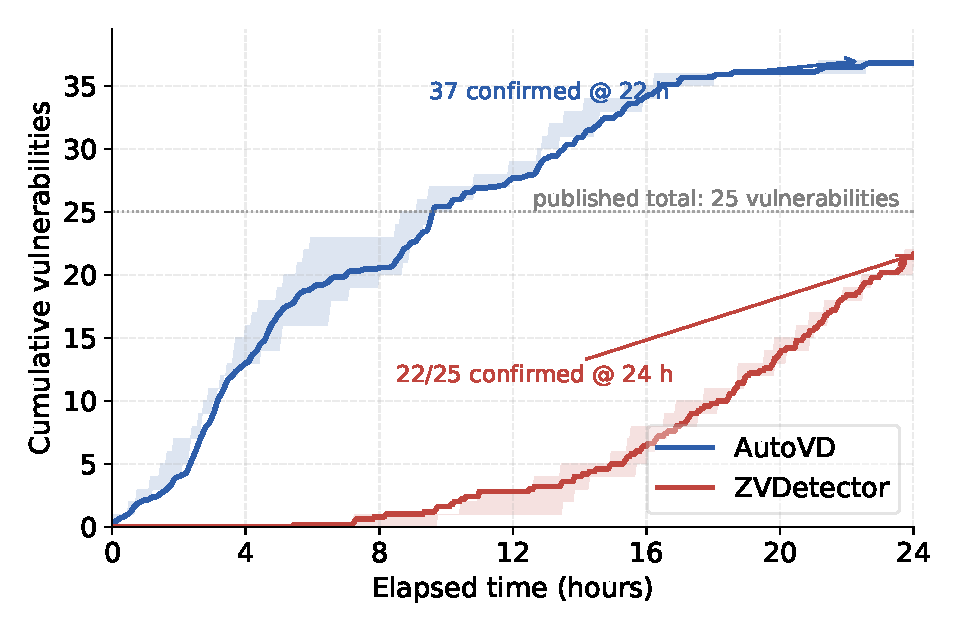
\includegraphics[width=\columnwidth]{figure/discovery_curve.pdf}
  \caption{Efficiency comparison under matched 24-hour budgets: cumulative confirmed vulnerabilities across the target set over per-device elapsed time (means of ten complete campaign replicates with run-level uncertainty). The dashed line marks the reference set of 25 findings~\cite{zvdetector}. AutoVD reproduces the reference set early and continues to additional faults, while ZVDetector leaves part of it unconfirmed at the budget boundary.}
  \label{fig:discovery-curve}
\end{figure}

\parab{Generation quality under the matched budget (\rq{5}).}
Figure~\ref{fig:generation-quality} summarizes the construction quality of the
tests generated within the 24-hour budget. Of the 1,983 generated plans, 1,949
(98.29\%) passed the Result Checker at first submission, a check-failure rate of
1.71\%. Only 8 approved plans were duplicates (0.41\% of valid). Both rates are
below the acceptance targets of 2.5\% and 1\%, respectively. Of the 34
rejections, 24 (70.6\%) are planning defects: state-contract violations (11),
order or step-budget overruns (7), and mutation mismatches (6). The remaining 10
are target or interface incompatibilities (5) and payload or encoding errors
(5). Most rejections therefore come from inconsistencies between a plan and its
declared state or mutation, not from malformed inputs. By construction, a
deliberately malformed payload that matches its declared mutation passes the
checker and remains eligible for execution. Overall, 1,941 of the generated
plans (97.88\%) are unique and checker-approved, so the matched budget yields
almost exclusively distinct state-conditioned tests rather than rejected or
repeated ones.

\begin{figure}[t]
  \centering
  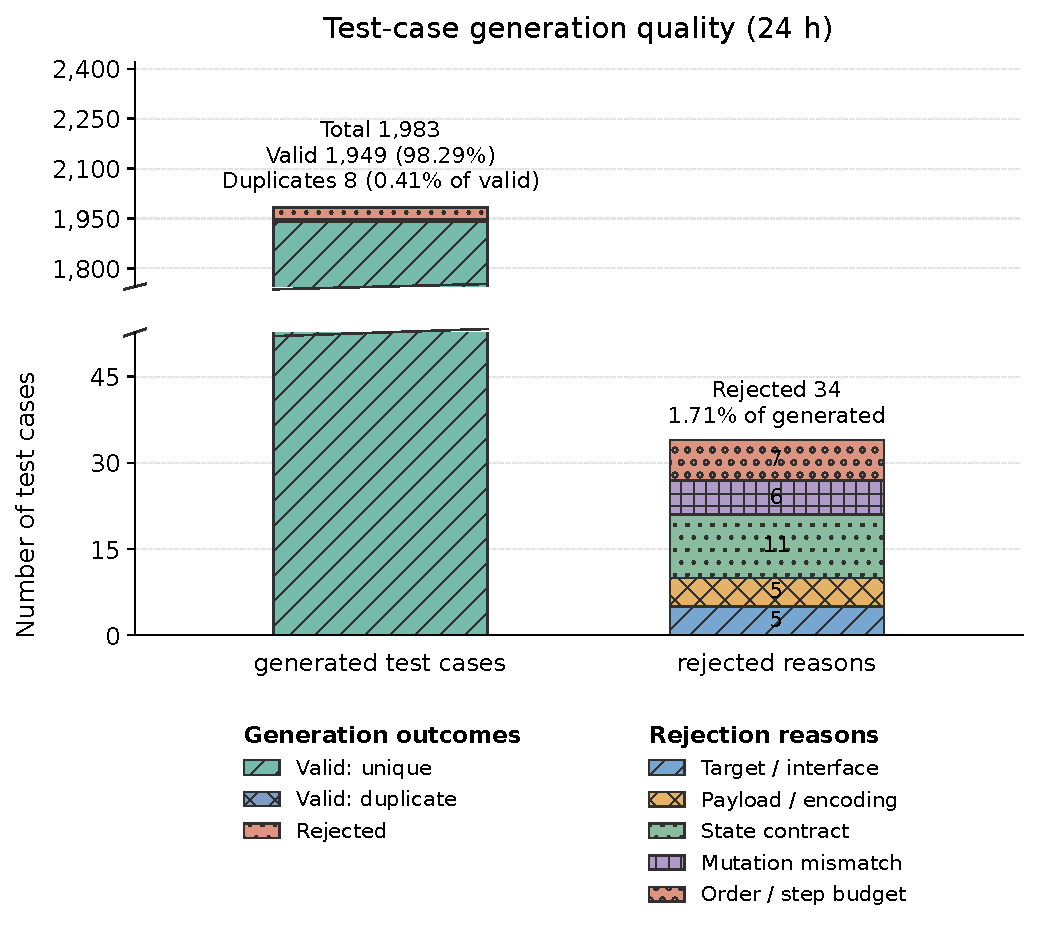
\includegraphics[width=\columnwidth]{figure/test_case_quality_typical.pdf}
  \caption{Test-case generation quality over the 24-hour campaign.
  Left: outcomes of all 1,983 generated tests (unique valid, duplicate valid,
  and rejected). Right: first-check rejection reasons for the 34 rejected tests.
  The y-axis is broken to show both scales. The check-failure rate (1.71\%) and
  duplicate rate (0.41\% of valid) are below the 2.5\% and 1\% targets.}
  \label{fig:generation-quality}
\end{figure}


\subsubsection{Ablation study.}

\parab{Combined-state ablation.}
Table~\ref{tab:reference-state-ablation} shows that the protocol-only configuration found 15 vulnerabilities. Device attributes increased this to 23, and permission analysis to 25~\cite{zvdetector}. Individual comparisons reported two single-message findings for each of B3 and B4, twelve dependency-based findings for B2, and ten correlation-based findings for B1. Agent ablations keep the awareness artifacts fixed to isolate planning, memory, and scheduling.

\begin{table}[t]
\centering
\caption{ZVDetector combined-state ablation~\cite{zvdetector}. Dependency and correlation columns use one relationship type, while Joint uses both.}\label{tab:reference-state-ablation}
\small
\begin{tabularx}{\columnwidth}{@{}X r r r r@{}}
\toprule Device-state support & Single & Dep. & Corr. & Joint \\ \midrule
None & 8 & 12 & 11 & 15 \\
Attribute collection & 12 & 16 & 19 & 23 \\
Attributes + permissions & 12 & 16 & 21 & 25 \\ \bottomrule
\end{tabularx}
\end{table}

% Ablation values are written directly below; data_status: placeholder.
\begin{figure*}[t]
  \centering
  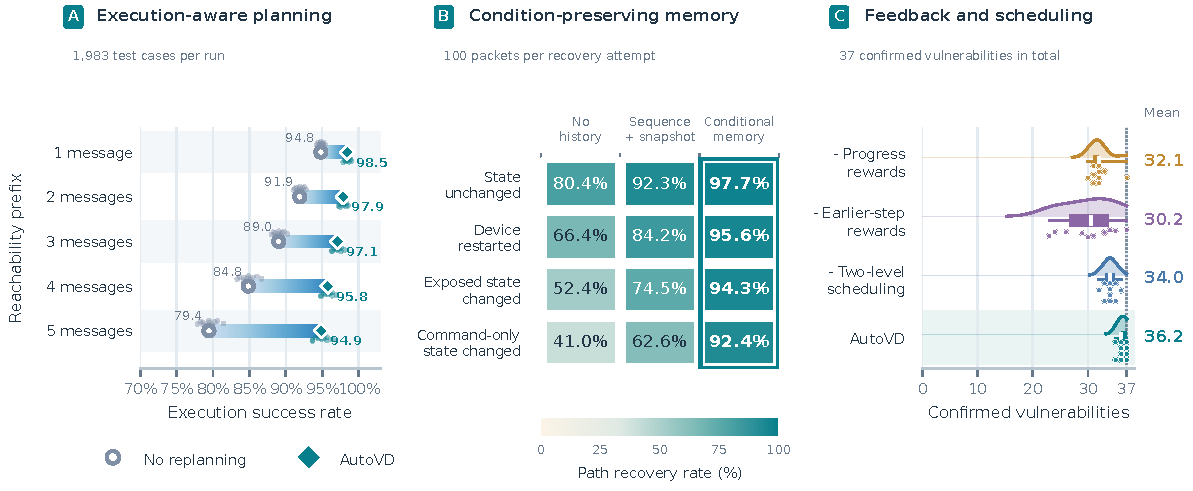
\includegraphics[width=\textwidth]{figure/ablation_study_combined.pdf}
  \caption{Agent ablations under matched 24-hour and 1{,}983-test-case per-device limits. (A) Mutation execution success by prefix length; small dots are run-level rates and large markers are means. (B) Path recovery under four initial-state conditions, with at most 100 delivered packets per recovery attempt. (C) Distinct vulnerabilities found from a fixed 37-item inventory. Each dot is one complete run over all 14 devices; repeated triggers of the same inventory item count once. Thick bars show interquartile ranges, white marks medians, and thin lines observed ranges over ten runs.}
  \label{fig:ablation-study}
\end{figure*}

Figure~\ref{fig:ablation-study} isolates adaptive planning and conditional memory (\rq{4}), and feedback-guided scheduling (\rq{5}). All variants share the protocol graph, attribute descriptors, mutation tools, model, and observation rules. Each comparison changes only the named mechanism, under a common 1{,}983-test-case reference workload and 24-hour limit per device. Rates are averaged over ten runs.

\noindent\textbf{[Without Adaptive Planning] (\rq{4})}:
The \emph{No replanning} variant follows a fixed analysis--setup--mutation sequence, keeping the checker and frozen memory corpus unchanged. Both variants receive 1{,}983 test cases per run, with per-test-case limits of 50 delivered packets and eight model rounds. The generation reference contains 1{,}949 checker-approved test cases (98.29\%); execution success additionally requires verified preconditions and confirmed mutation delivery. Rejected test cases and failed setup remain in the denominator. Figure~\ref{fig:ablation-study}(A) shows that the gap increases from 3.7 to 15.4 percentage points between one- and five-message prefixes. Replanning can correct failed setup or an unexpected intermediate state before mutation.

\noindent\textbf{[Without Conditional Memory] (\rq{4})}:
We retain historical sequences and state snapshots but remove their applicability conditions and executable setup. A no-history variant reconstructs paths for the same target test cases. Current-state checks and adaptive planning remain enabled. Each run distributes 1{,}983 recovery attempts across four session conditions. Each attempt allows at most 100 delivered packets in total, including setup, path execution, and state probes. Recovery fails if the required conditions and target path cannot be verified within this budget. In Figure~\ref{fig:ablation-study}(B), conditional memory recovers 92.4\% of paths after command-only state changes, compared with 62.6\% for sequence-and-snapshot storage. The retained setup restores conditions that a historical snapshot cannot establish in the new session.

\noindent\textbf{[Feedback and Scheduling] (\rq{5})}:
The \emph{$-$ Progress rewards} variant removes bonuses for observable exploration progress, including new states and transitions. The \emph{$-$ Earlier-step rewards} variant removes backward event-reward allocation: the event value remains with the decision where the failure becomes visible, and earlier contributing decisions receive none of that value. The \emph{$-$ Two-level scheduling} variant replaces context-specific two-level UCB with uniform selection of feasible state--message opportunities and one shared UCB pool for mutation strategies and modes across contexts. \system{} retains both feedback components and selects opportunities and mutations at separate, context-specific levels. Planning, memory, confirmation rules, and replay budgets remain unchanged. Figure~\ref{fig:ablation-study}(C) counts distinct findings from the fixed 37-item inventory across all 14 devices in each of ten complete runs. \system{} averages 36.2 findings, compared with 32.1, 30.2, and 34.0 for the three ablations, respectively. Repeated triggers count once, and no run can exceed the inventory size.

\section{Related Work}\label{sec:related-work}
\parab{Combined-state and specification-assisted fuzzing.}
ZVDetector discovers message relationships and command-accessible attributes to explore correlated protocol and device states~\cite{zvdetector}. It retains triggering sequences with state snapshots and prioritizes nearby combined states after anomalies. Our focus is the applicability and feedback ownership of an agent-generated experiment. \system{} binds each proposed test to checked execution conditions, retains those conditions for cross-session reuse, and revises original experiment utilities through conserved delayed-event feedback.

LLMIF uses specification-augmented reasoning to interpret responses and extend useful sequences~\cite{llmif}. mGPTFuzz generates state machines from the Matter specification and checks response and attribute behavior against them~\cite{mgptfuzz}. Both therefore go beyond one-shot input generation. Our focus is on how a continuing campaign retains applicability conditions and revises the utility of original experiments when evidence arrives later. This distinction must be evaluated under shared protocol knowledge rather than attributed merely to using an LLM.

\parab{Reuse in black-box vulnerability detection.}
IoTBec matches externally visible interfaces against signatures derived from known vulnerability reports and generates directed tests for recurring faults~\cite{iotbec}. Its reuse unit is a vulnerability/interface signature. Our reuse unit is a state-conditioned experiment with an executable setup and sequence. These approaches address different information sources and need not be substitutes. IoTBec's detector uses black-box interface observations, although its reported evaluation executes vulnerability tests in emulated environments. Such results are not evidence that the same radio-level workflow has been evaluated on unmodified physical devices.

\parab{Agent-assisted firmware analysis.}
MALF coordinates protocol-testing agents and retrieves historical strategies~\cite{malf}. Our distinction is the applicability record and feedback ownership of a state-conditioned experiment, rather than coordination or retrieval alone. FirmAgent uses fuzzing-derived input points for LLM-assisted taint analysis and proof-of-concept refinement~\cite{firmagent}. PANGOLIN recovers interfaces and parameter specifications across script and binary components and corrects them using responses~\cite{pangolin}. Both FirmAgent and PANGOLIN use firmware code or a rehosted runtime. In contrast, \system{} relies on checked protocol observations and replay to support test applicability and sequence contribution on unmodified devices.

\parab{Firmware fuzzing and scheduling.}
Rehosting-based systems such as FIRM-AFL and Fuzzware obtain coverage from an executable firmware environment~\cite{firmafl,fuzzware}. Hoedur restructures firmware inputs into typed streams and uses bandit-based stream scheduling~\cite{hoedur}. Thus applying a bandit policy to fuzzing is not new. Our scheduling question is whether a state--message context and its mutation choices should be compared separately under progress and delayed utility revisions. Static systems such as KARONTE, SaTC, and Operation Mango recover flows from firmware~\cite{karonte,satc,mango}, while N\"{U}WA checks inconsistent input constraints~\cite{nuwa}. These methods can supply complementary evidence when firmware is available, but their code-level measurements are not directly observable in our black-box campaigns.

\section{Discussion}\label{sec:discussion}
\parab{What black-box evidence can establish.}
A stable signature summarizes observable state rather than the complete internal device state. Different hidden states can share a signature and still behave differently under later messages. Consequently, coverage measures apply to the observed abstraction. Reproduction supports a repeatable fault under stated conditions, while memory corruption, exploitability, and root-cause identity require additional evidence. These limits constrain both the interpretation of progress and the strength of vulnerability claims.

\parab{Contribution under imperfect replay.}
Replay-supported weights depend on matched baselines and executable ablations. Removing an early setup can invalidate an entire sequence, in which case its contribution remains unresolved rather than becoming proof of necessity. Timing-sensitive failures and persistent state may make matched replay impossible. The method then retains uncertainty and provisional evidence instead of fabricating backward credit. The single-budget rule prevents repeated alarms from multiplying value, but can underrepresent multiple independent faults within one episode. Fault triage should use separately restored baselines where possible.

\parab{Adaptation and model dependence.}
An LLM may propose unsupported operations or inconsistently use retrieved evidence. Checking target compatibility and test intent reduces these errors but cannot make semantic planning complete. Protocol documents, responses, and retrieved records are untrusted evidence, not instructions that can authorize tool use. The execution boundary should enforce the campaign's permitted operations and resource limits independently of model output. Model versions and prompt changes also require separate measurement because they can change exploration behavior.

\parab{Transfer and operational limits.}
Reusing the planning and feedback interfaces for another protocol requires validated schemas, state-access methods, and a gateway adapter. It does not follow from prompt portability alone. Cross-version memory likewise requires revalidation of stored conditions. Pairing and physical recovery may still require an operator. A device that cannot be safely restored limits both exploration and the evidence available for comparison.

\parab{Testing ethics.}
The authorized, isolated setting in Section~\ref{sec:threat-model} limits the operational scope but does not eliminate the risk of persistent device failure. Destructive tests require a documented recovery plan and stopping rule. Devices attached to safety-critical processes are not ordinary fuzzing targets. Confirmed findings require reproducible evidence and coordinated disclosure. Vendor confirmation and disclosure are not claimed as completed in the current draft.

\section{Conclusion}\label{sec:conclusion}
This paper presents \system{}, an agent-guided black-box fuzzing framework for uncovering IoT vulnerabilities triggered by combined protocol and device states. The framework integrates message relationships and device attributes to guide LLM agents in generating mutation sequences and verifying their execution conditions. Conditional memory retains executable setup and applicability conditions for test reuse, while long-horizon feedback and contextual scheduling guide continued exploration. Experiments on Zigbee and Z-Wave devices demonstrate that \system{} effectively extracts protocol message formats, identifies message relationships, and characterizes device attributes. By combining state awareness, conditional reuse, and adaptive exploration, \system{} generates tests that accelerate vulnerability discovery and reveal diverse state-dependent corner cases.

\section*{Acknowledgment}
% TODO: Add acknowledgments and funding information after de-anonymization.

\bibliographystyle{IEEEtran}
\bibliography{references}

\end{document}
